% Project Proposal Document
\documentclass[final]{cmpreport}
\makeatletter
\input{t1pcr.fd}
\makeatother
\setlength{\footnotesep}{3ex}
\title{\Codex: evaluating Agile Solo by developing a Web App for table-top role-playing games}
\author{Christopher Alastair Irvine}
\registration{100036248}
\supervisor{Dr Katharina Huber}
\ccode{CMP-6013Y}
\summary{The \Codex \ project was designed to evaluate a single developer Software Engineering Agile methodology, known as Agile Solo, by implementing this methodology into the development life cycle of a web app. The front-end of the web app was developed using ReactJS whilst the back-end contained a Node.js server and a MySQL database. Throughout the development of the \Codex \ web app, the developer maintained a journal that detailed the experience of using Agile Solo within the development life cycle. The developer additionally used the journal to suggest adjustments to the Agile Solo methodology based on those experiences. The development of \Codex \ was not without flaws and ultimately was completed as a challenged project, through the Standish Group Chaos Report classification system. The evaluation of Agile Solo, supported by evidence from the journal kept by the developer, revealed that Agile Solo was suited towards a single developer project. The methodology was instrumental in the management of the project, providing the developer with the confidence and security that was necessary to continue development. The developer did suggest that the methodology could be improved through the inclusion of stand up meetings once adapted from the Scrum methodology.}
\acknowledgements{
	I would like to thank Dr Katharina Huber for taking on the supervision of this project. Additionally, I would like to thank Wizards of the Coast for their generosity and kindness in allowing the use of their Intellectual Property and Assets for this project.
}
\usepackage{rotating}
\usepackage{csquotes}
\usepackage{hhline}
\usepackage{caption}
\usepackage{makecell}
\usepackage{listings}
\newcommand{\ueacmp}{UEA School of Computing Sciences}
\newcommand{\WotC}{Wizards of the Coast}
\newcommand{\dnd}{D\&D}
\newcommand{\sem}{Software Engineering Model}
\newcommand{\sems}{Software Engineering Models}
\newcommand{\Codex}{\textsc{Codex}}
\newcommand{\AgileSolo}{\emph{Agile Solo}}
\graphicspath{ {Images/} }
\lstdefinelanguage{JavaScript}{
	keywords={typeof, new, true, false, catch, function, return, null, catch, switch, var, if, in, while, do, else, case, break},
	keywordstyle=\color{blue}\bfseries,
	ndkeywords={class, export, boolean, throw, implements, import, this},
	ndkeywordstyle=\color{darkgray}\bfseries,
	identifierstyle=\color{black},
	sensitive=false,
	comment=[l]{//},
	morecomment=[s]{/*}{*/},
	commentstyle=\color{purple}\ttfamily,
	stringstyle=\color{red}\ttfamily,
	morestring=[b]',
	morestring=[b]"
}
\lstset{
	language=JavaScript,
	backgroundcolor=\color{lightgray},
	extendedchars=true,
	basicstyle=\footnotesize\ttfamily,
	showstringspaces=false,
	showspaces=false,
	numbers=left,
	numberstyle=\footnotesize,
	numbersep=9pt,
	tabsize=2,
	breaklines=true,
	showtabs=false,
	captionpos=b
}
% EOF Preamble and Macros
	
% BOF Document
\begin{document}	
	% BOF Introduction
	\section{Introduction} \label{sec:introduction}
	This paper is to serve as the report for the \Codex \ project. \Codex \ possess two distinct, yet related, components. Firstly, \Codex \ aimed to research, implement and assess a single developer Software Engineering Agile methodology. This would be evaluated throughout the development of the second component of \Codex, a web app (see Section \ref{sec:web-app}) that was based on the game of Dungeons and Dragons (\dnd). 
	
	\dnd, at the time of writing, was a popular table-top role-playing game published by \WotC. In the game, a team of players would work together to overcome a series of challenges created by another player known as the Dungeon Master (DM). From these challenges, a narrative would form, which in turn would create a campaign. For a full explanation of \dnd \ see Section \ref{sec:what-dnd} and the ``Dungeons and Dragons Explained" document found within the supporting documents folder for the \Codex \ project. 
	
	Software Engineering, at the time of writing, was a technical discipline within the field of Computer Science that aimed to apply scientific and technical knowledge to the development of software. This would be implemented through the application of a methodology that would manage the development time and tasks (see Section \ref{sec:what-se}). The Agile Manifesto was created to address a crisis within the Software Industry, which was suffering from a large number of failed projects in the 1980s and 90s. For example, the Agile Manifesto encouraged developers to decrease the importance of contracts that would lock clients into a potentially flawed piece of software. Developers instead favoured inviting the clients to take part in the development process, thus ensuring the final product satisfied the clients. However, Agile does recognise the importance of contracts within commercial software development (see Section \ref{sec:what-agile}). Two single developer methodologies that were identified as potential candidates: Agile Solo (see Section \ref{sec:agile-solo}) and XP for One (see Section \ref{sec:xp-for-one}). Both of these methodologies were inspired by already successful team methodologies; Scrum and Kanban in the case of Agile Solo and ExtremeProgramming (XP) inspiring XP for One. 
	
	The front-end of the \Codex \ web app was developed in ReactJS, a JavaScript Library for building user interfaces (see Section \ref{sec:react-js}) whilst the back-end utilised a Node.js server and MySQL database (see Section \ref{sec:backend}). The combination of front-end and back-end technologies would form a \emph{stack} (see Section \ref{sec:stack}). The development of \Codex was influenced by the preliminary design work completed by the developer, a summary of which can be found in Section \ref{sec:design}. A full design document for the \Codex \ web app is present within the supporting material. However, the development was not without issue. These issues, as described in Section \ref{sec:dev-obs}, and subsequent solutions, found in Section \ref{sec:dev-eval}, caused the development of the \Codex \ web app to be completed with a challenged status. This classification was based on the Standish Group Chaos Report (see Section \ref{sec:feedback}).
	
	Despite the development issues, the Agile Solo framework was implemented without hindrance (see Section \ref{sec:use-agile-solo}), allowing for the evaluation of the methodology to be executed later in this report (see Section \ref{sec:agile-solo-eval}). 
	
	Figure \ref{gantt:pplan}, shows the Gantt Chart for the \Codex \ project, which was adhered to throughout the life cycle of the project, which has remained unchanged since the progress report. 
	
	\begin{cmpfigure}{\Codex \ Gantt Chart, outlining the major tasks and deliverables\label{gantt:pplan}}
		\begin{sideways}
			\newganttchartelement{voidbar}{
				voidbar/.style={draw=black, top color=black!25, bottom color=black!23
			}}
			\begin{ganttchart}[y unit chart = 0.75cm, y unit title = 0.75cm, x unit=0.45cm, vgrid, title label font=\scriptsize,
				canvas/.style={draw=black, dotted}]{1}{34}
				\gantttitle{Project schedule shown for e-vision week numbers
					and semester week numbers}{34} \\
				
				\gantttitlelist{8,...,41}{1}\\
				\gantttitlelist{1,...,12}{1} \gantttitle{CB}{4}
				\gantttitlelist{1,...,9}{1} \gantttitle{EB}{4}
				\gantttitlelist{10,...,14}{1}\\
				
				%The elements, bars and milestones, are identified as elem0, elem1, etc.
				\ganttbar{Project Proposal}{1}{2} \\        		%elem0  
				\ganttbar{Literature Review}{2}{5} \\      			%elem1 
				\ganttmilestone{Literature Review Finished}{5} \\	%elem2
				\ganttbar{Design 1}{4}{8} \\ 						%elem3
				\ganttbar{Development 1}{9}{11} \\					%elem4
				\ganttbar{Progress Report}{11}{12} 					%elem5
				\ganttmilestone{}{12} \\							%elem6
				\ganttbar{Development 2}{11}{16} \\  		 		%elem7
				%week 1 of semester 2 is the 17th week in schedule 
				\ganttbar{Report Writing 1}{17}{19} 	        	%elem8
				\ganttmilestone{}{19} \\							%elem9
				\ganttbar{Design 2}{19}{20} \\      				%elem10
				\ganttbar{Development 3}{21}{26} \\					%elem11
				\ganttbar{Testing}{24}{26} \\						%elem12
				\ganttmilestone{Code Delivery}{26} \\       		%elem13
				\ganttbar{Report Writing 2}{27}{30} \\  			%elem14
				\ganttbar{Demonstration preparation}{31}{34}   		%elem15
				
				\ganttlink{elem0}{elem1} \ganttlink{elem1}{elem2} \ganttlink{elem2}{elem3}
				\ganttlink{elem3}{elem4} \ganttlink{elem4}{elem5} \ganttlink{elem5}{elem6}
				\ganttlink{elem6}{elem7} \ganttlink{elem7}{elem8} \ganttlink{elem8}{elem9} \ganttlink{elem9}{elem10}
				\ganttlink{elem10}{elem11} \ganttlink{elem11}{elem12} 
				\ganttlink{elem12}{elem13} \ganttlink{elem13}{elem14}
				\ganttlink{elem14}{elem15}
			\end{ganttchart}
		\end{sideways}
	\end{cmpfigure}	

	\section{What is \Codex?} \label{sec:what-codex}
	\Codex \ was a project with two components. The first, produced a web app built in ReactJS that was developed using a single developer Software Engineering Agile methodology, the second component was to evaluate the quality of that methodology. By the end of this section, we will have an appreciation of the \Codex \ web app, in terms of both context and purpose (see Sections \ref{sec:context}).
	
		\subsection{Context} \label{sec:context}
		The \Codex \ web app was based around the popular tabletop role-playing game known as Dungeons and Dragons (\dnd), created and published by \WotC. This game, and the principles that bring the game to life drove the requirements, which formed the basic structure of the \Codex \ web app. Therefore, in order to understand the functionality, principle and importance of the \Codex \ web app, we must first gain an understanding of \dnd. 
		
		The author of this paper has multiple years of experience with \dnd, both as a \emph{Player} and \emph{Dungeon Master} (DM). The \Codex \ web app began as a personal project for the author of this paper, which grew into a tool to evaluate a single developer Software Engineering Agile methodology. 
		
			\subsubsection{What is Dungeons and Dragons?} \label{sec:what-dnd}
			The game of \dnd, at time of writing, was a popular table-top role-playing game where a group of friends would have engaged in a grand fantasy adventure (\cite{DnDOriginal}, \cite{DnDHistory}). The story would be divided into manageable blocks of time known as \emph{sessions}. Each session may take between two and four hours to run, however, this was not strictly enforced and would be decided by the group of players. The events of each session, and the larger campaign, was created and controlled by a player known as the \emph{Dungeon Master} (DM) (for more details on DMs please see Section \ref{sec:dm-vs-player}). However, the campaign would not always adhere to the plans of the DM. The players, who were clueless as to the next plot in the campaign, might take the story in an entirely different direction several times a session. The DM would have to react to these unexpected inputs and redraw the narrative during each session or attempt to subtly guide the players back on track \citep{PlayerHandbook}. 
			
			It was possible for DMs to purchase pre-written campaigns, published either by experienced DMs or \WotC. Many DMs would take it upon themselves to create their own worlds (sometimes referred to as settings) in which the campaign would occur or alter the pre-written campaigns to suit the needs of the group. Every game of \dnd \ was inherently different from each other, including those following the same campaign book. Because of this difference, it was hard to estimate how many sessions a campaign might take. 
			
			The players would form an entity known as the \emph{party}, that would consist of the characters that the players embodied for the duration of the campaign. Each player controls one character, known as a \emph{player character} (PC), within the party. The party would serve as the device for interaction with the world, this is also true for the DM who would not embody one character, but multiple characters within the setting. These characters would be referred to as \emph{non-player characters} (NPC) and would include both allies and enemies of the party. For that reason, the external perception of the \dnd \ might be that the players would be against the DM. Nothing could be further from the truth, as it was the relationship that existed between the players and the DM that would shape the outcome of the campaign \citep{DnDPeople}.
			
			\begin{figure}[h] 
				\begin{subfigure}{0.5\textwidth}
					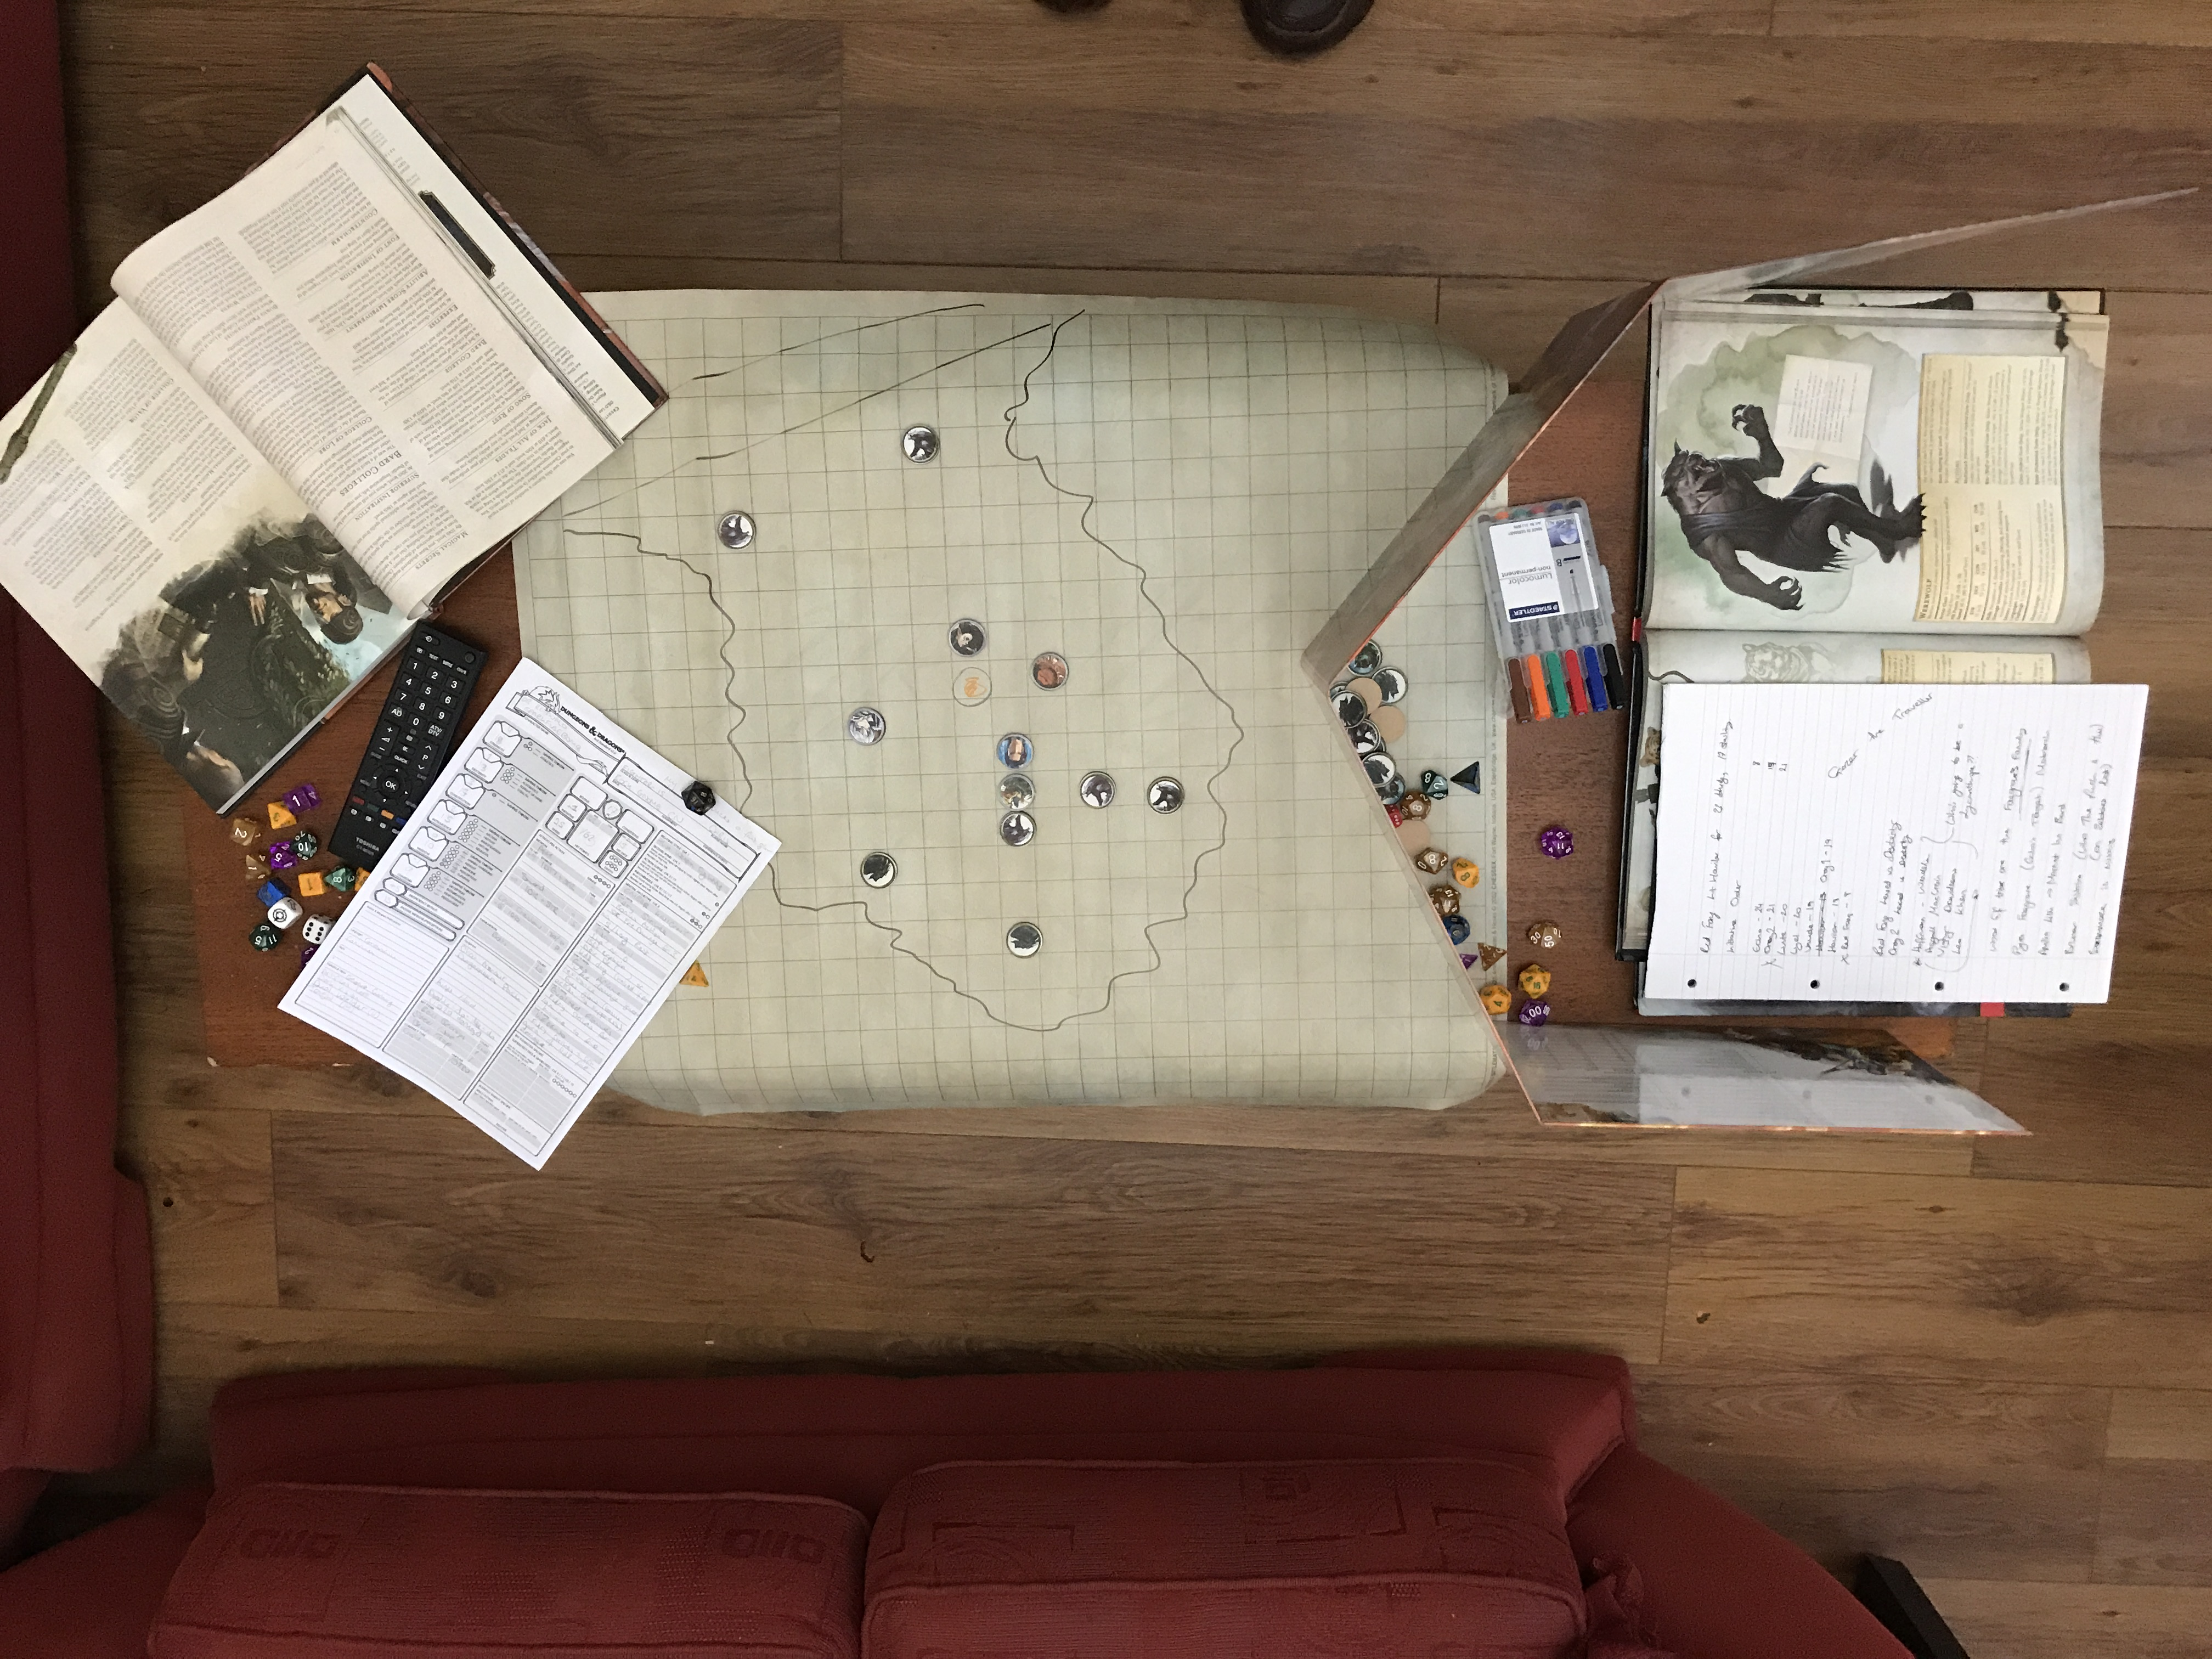
\includegraphics[width=\linewidth, height=5cm, angle=180]{DnD_Live.jpg}
					\caption{A typical \dnd \ set up. From left to right: DM note pad on top of a couple of official \WotC \ core books (\emph{Monster Manual} shown), set of dice, a gridded battle mat and tokens, a player character sheet, player's set of dice and the \WotC \ \emph{Players Handbook}} \label{fig:DnDLive}
				\end{subfigure}
				\begin{subfigure}{0.5\textwidth}
					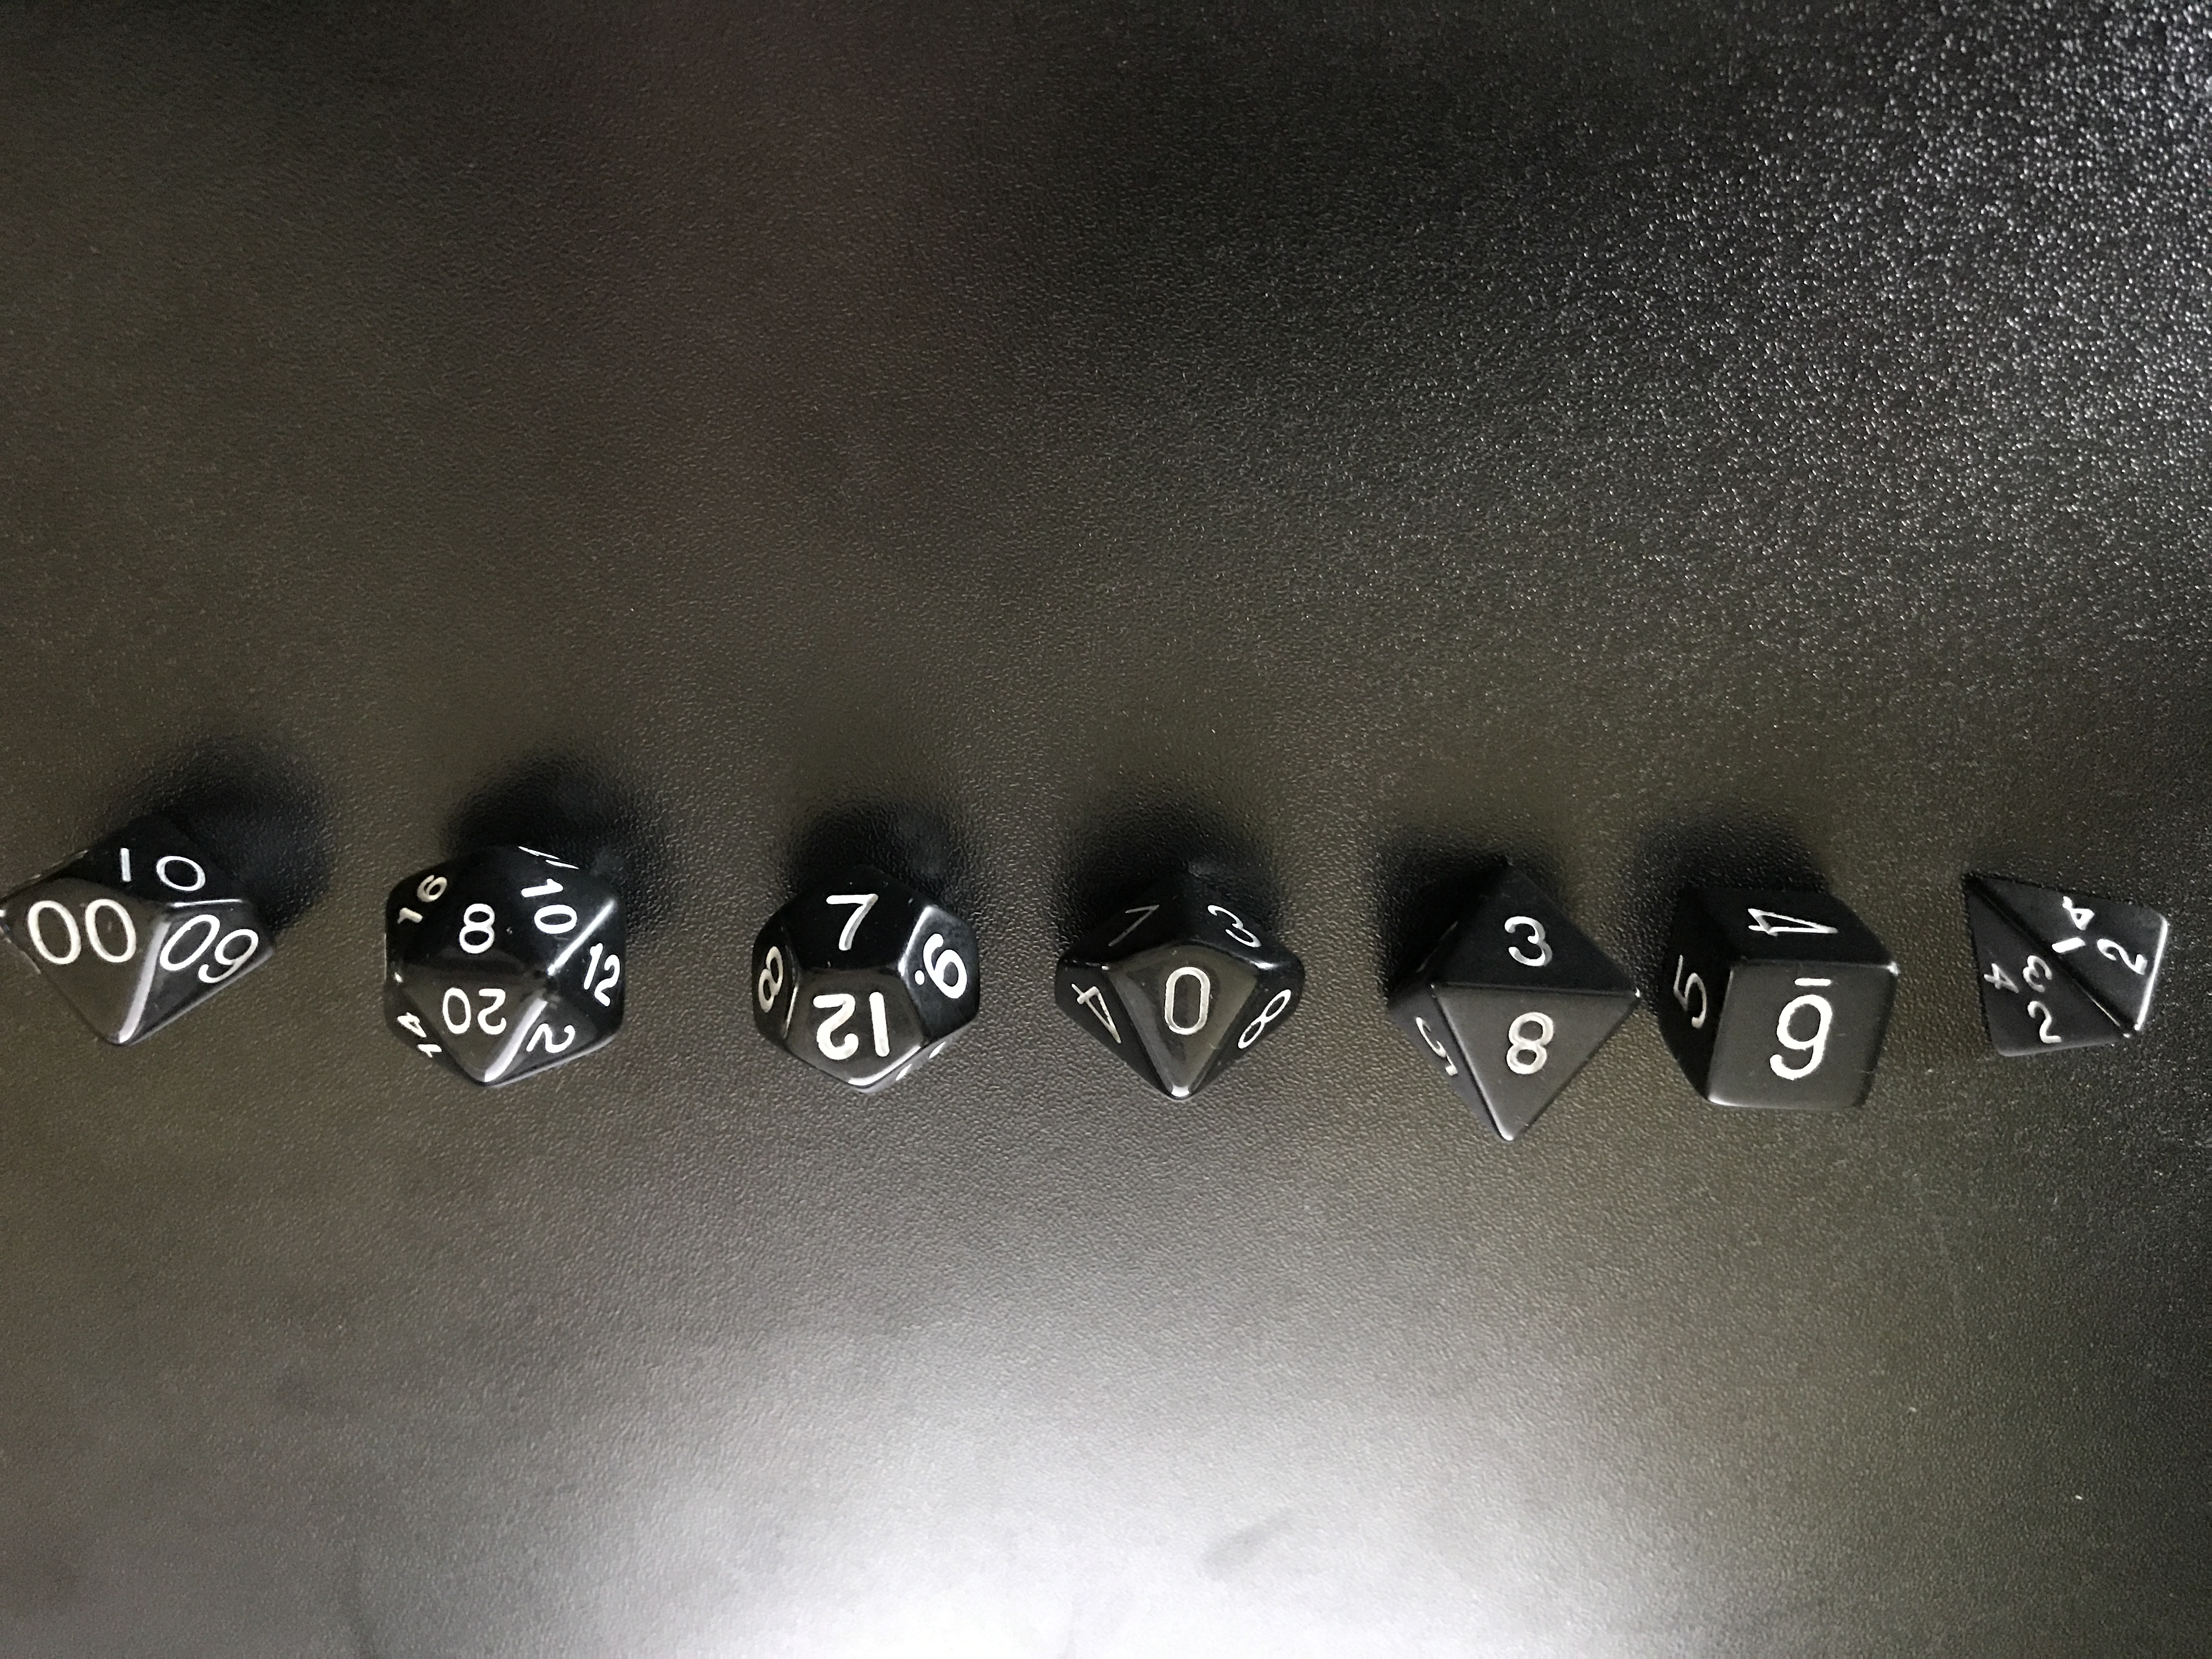
\includegraphics[width=\linewidth, height=5cm, angle=180]{DnD_Dice.jpg}
					\caption{An example set of dice that was needed to play \dnd. From left to right: 4-sided, 6-sided, 8-sided, 10-sided, 12-sided, 20-sided and a 10-sided dice in increments of 10s} \label{fig:DnDDice}
				\end{subfigure}
				\caption{The above examples reflect the typical equipment that would be used in a game of \dnd.} \label{fig:dnd-equipment}
			\end{figure}
			
			Despite the complicated nature of \dnd \ the equipment that was needed to play the game was minimal. A group of players would only have needed a single set of dice, a copy of the core books (\emph{Dungeon Master's Guide \citep{DMGuide}, Players Handbook and Monster Manual \citep{MonsterManual}}), a set of character sheets (1 per player), pens and paper. Everything else, such as more dice, a \emph{Dungeon Master Screen}, Campaign Books, a gridded Battle Mat and Tokens were supplementary. The dice that was used for \dnd \ are as follows; twenty-sided, twelve-sided, two ten-sided (one in increments of one, the other in increments of ten), eight-sided, six-sided and four-sided. Figure \ref{fig:DnDLive} is an example of what a \dnd \ table might have looked like, whereas Figure \ref{fig:DnDDice} is an example of the different dice used for \dnd \footnote{When discussing these dice further in this paper, they will be referred to as d\emph{X} where \emph{X} is the number of sides the dice has (for example the twenty-sided dice is referred to as \emph{d20}). The exception to this is the secondary d10 (which has increments of 10) which is referred to as the \emph{d100}.}.
			
			Throughout the campaign, the party would have to face many challenges designed by the DM. These challenges might be full-scale battles involving multiple powerful enemies and allies, to small-scale skirmishes between only a handful of characters. Alternatively, challenges could be a non-combat encounters where the party would have to negotiate themselves out of a tight situation with the law, or to circumvent a magical trap set by an ancient being in order to acquire an item of treasure. The effectiveness in which the party would handle these situations is decided through a simple mathematical system. 
			
			Every character within a \dnd \ world would have had a set of \emph{attributes} that would dictate how that character interacted with the environment around them. These attributes are; \emph{strength}, \emph{dexterity}, \emph{constitution}, \emph{intelligence}, \emph{wisdom} and \emph{charisma} (more details of these attributes are available the ``Dungeons and Dragons Explained" document found in the supporting documents). These attributes were rated between one and twenty, with twenty being the highest a character could achieve without magical augmentation in the game. The score would be divided by 10, rounding up to the nearest whole number, creating an \emph{ability modifier} which would be applied to the roll a dice (we should note that this number could be negative). If a character was highly skilled in a particular task, then a \emph{proficiency bonus} would also be applied. This calculation is summarised in the below equation \ref{eq:skill-check}. 
			
			\begin{equation} \label{eq:skill-check}
			skill \ check = d20 + ability \ modifier + proficiency \ bonus
			\end{equation}
			
			These skill checks allowed the players to interact with the world, via the player character, in a quantitative manner. The higher a skill check, the better that character performed in that challenge. Challenges would have a \emph{difficulty class}, an arbitrary number which indicates the level of skill (or luck in some cases) needed to perform that task. If the challenge was to strike an enemy, for example, it would be easier to wound a bandit wearing no armour than it would be to wound a skilled warrior in plate armour. 
			
			Winning a game of \dnd \ was not a simple manner, as there were no set win conditions. It depended entirely on the campaign that was being run by the DM. A typical example might be that the party were a group of loyalists who were tasked with overthrowing a usurper and restoring the rightful monarch to the throne. That party would \emph{win} were they to do so, however, the objectives might change were the party to learn of some new, unsavoury, information about their beloved monarch. A campaign might end without achieving the original goal, or shorter campaigns may end with the start of a new story for the party. It all depended on the attitude of the players towards the game.
			
			A short, worked example of \dnd \ may be found within the supporting materials for this report.
			
			\subsubsection{How does a Dungeon Master differ from a Player?} \label{sec:dm-vs-player}
			In Section \ref{sec:what-dnd}, we explored some of the principles that gave \dnd \ life, however, the most important principle to the \Codex \ web app was the difference between the DMs and Players. As briefly explained above, a DM was a member of the group who would control the narrative of the campaign and dictated what was occurring during each session. Whilst the DM may write the campaign narrative they would not control how the story unfolded. Ownership of the narrative ultimately belonged to the group as a whole. Player input during the sessions shaped the world and story as the party progressed through the campaign, forming relationships with characters that the DM portrayed. 
			
			It was the responsibility of a DM to ensure that the party was enjoying the campaign, narrative and challenges. As a result, the DM needed to have know every intricacy of the world at any given time, or be able to improvise when they did not know the answer. As only a DM could bring a world to life. Therefore the amount of information that a DM would have to deal with would have been immense. Every DM would have a folder (either physical or digital) containing notes on places, people and events that resided within the world. This folder would not only contain the events of the past, but additionally the plans for the future. Skilled DMs would rely on their folder more than any other resource during a session to ensure the delivery of the appropriate reaction to party input. The maintenance of a DM folder was costly in both time and effort \citep{GMTips}. Whilst there was no definitive time spent in order to prepare for a session, DMs could easily spend over ten hours a week planning for their \dnd \ campaign \citep{DungeonMaster}. 
			
			However, DMs were a part of the game just like the players were. \dnd \ was never the party against the DM, instead, it was a symbiotic relationship where they would explore the world together and share the experience. Whilst a DM knew what was planned to happen next, it was decided by the players what actually occurred. 
				
			\subsubsection{Why was the \Codex \ web app developed?} \label{sec:why-codex}
			As mentioned in Section \ref{sec:context}, \Codex \ began as a personal project for the author of this paper. The original functionality of the app was to be a platform for tracking combat during games of \dnd. Since then the functionality of the \Codex \ web app has grown to include a note taking system and several other minor features that will be discussed in Section \ref{sec:dev-and-imp}. Whilst there are several other systems (explored in Section \ref{sec:other-dnd-apps}) that assists the DM, they often only perform one task. The \Codex \ web app aimed to be the assistance app of choice for DMs as the system possessed a wide range of functionality. DMs spend a lot of time and effort in running their games of \dnd \ (as discussed in Section \ref{sec:dm-vs-player}). The \Codex \ web app attempted to remove some of the more laborious high pressure tasks from DMs, thus making the game more enjoyable for the DMs.

	\section{Related Work} \label{sec:related}
	In this Section, we will explore the work that was pertinent to the \Codex \ project. We will have a greater appreciation of the \Codex \ web app, by evaluating the similar systems available at the time of writing, and gain an understanding of the Software Engineering discipline in addition to the Web-App architecture through the review of academic works.
	
		\subsection{Dungeon and Dragons Apps} \label{sec:other-dnd-apps}
		At the time of writing, there were several applications that existed to assist in the running of \dnd. These apps had varying levels of functionality, however, they differed from the \Codex \ web app. For example, the official \dnd \ Beyond app \citep{dnd-beyond} (discussed further in Section \ref{sec:dnd-beyond}), had a huge range of functionality including digital character sheets and a quick reference database. This service was aimed towards the players of the game, not towards the DMs, therefore \dnd \ Beyond does not support session planning and encounter generation\footnote{Encounter Generation was a feature of some \dnd \ apps, where either the User will generate an encounter manually or randomise the encounter using the system algorithms.} to the same level as the \Codex \ web app.
		
			\subsubsection{\dnd \ Beyond} \label{sec:dnd-beyond}
			\dnd \ Beyond was a web app that was developed by \emph{Curse, Inc.} and published by \WotC \ (the creators and owners of \dnd). The purpose of \dnd \ Beyond was to digitise the experience of \dnd \ without removing the table-top, social aspect (see Section \ref{sec:roll20}) of the game. However, \dnd \ Beyond was not just a web-app that held digital records of PCs. There was an additional emphasis on community and sharing amongst the Users through the use of Forums and the ability to publish individual content through the site. 
			
			\begin{figure}[H]
				\centering
				
\includegraphics[width=\linewidth]{dnd-beyond.png}
				\caption[\dnd \ Beyond homepage screenshot]{A screen shot of the \dnd \ Beyond web-app homepage (05/05/2018), showing the various functions of the service. We can see several articles (with more off-screen); separate sections for personal content, characters, compendium (campaign section), spells (see the Extended \dnd \ Explanation in portfolio for more details on spells), items, monsters, marketplace (where users may purchase electronic books to unlock content) and forums in the navigation bar. Additionally there were search, social media, chat and account functionality in the header of the screenshot.} \label{fig:dnd-beyond}
			\end{figure}
		
			Figure \ref{fig:dnd-beyond} was a screenshot taken from the \dnd \ Beyond homepage. Whilst a full description of the functionality of \dnd \ Beyond is available in the Design Document found in the supporting documents, it would be crucial to underline some of the key features of the service. Firstly, the ability to digitally store a Player Character (PC), with a full description of abilities and spells attached to that character was critical to many players, who were frustrated by the constant searching through the core rulebooks of the game. Secondly, \dnd \ Beyond gave the community the ability to directly share and use content created not by \WotC \ but by other players of the game. Whilst this was happening on alternative sites such as the \dnd \ Reddit Forum \citep{reddit-dnd} (a popular forum website), \dnd \ Beyond brought the community back to \WotC \ and centralised it. However, one of the largest downfalls of \dnd \ Beyond was the need for compulsory purchase of the \WotC \ books through the web-app, even if the user might own a physical copy already. Only by purchasing the book (potentially for a second time) could the user access the majority of the content on the web-app (see Figure \ref{fig:dnd-beyond-mm}).
			
			\begin{figure}[h] 
				\begin{subfigure}{0.5\textwidth}
					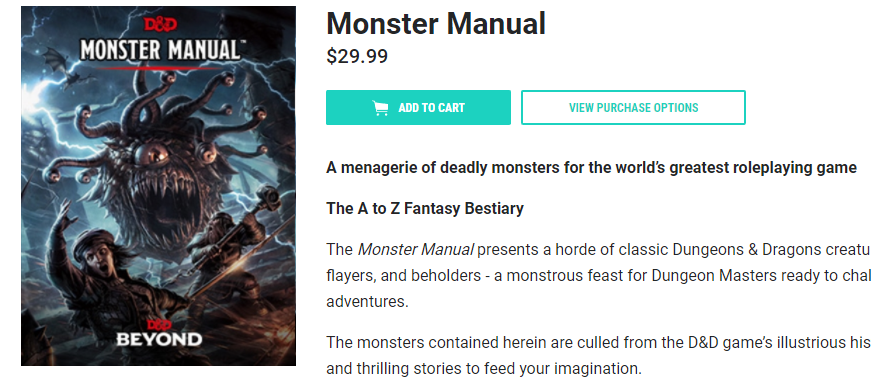
\includegraphics[width=\linewidth]{dnd-beyond-mm-purchase.png}
					\caption{\dnd \ Beyond \emph{Monster Manual}} \label{fig:dnd-beyond-mm}
				\end{subfigure}
				\begin{subfigure}{0.5\textwidth}
					
\includegraphics[width=\linewidth]{roll20-mm-purchase.png}
					\caption{Roll20 \emph{Monster Manual}} \label{fig:roll20-mm}
				\end{subfigure}
				\caption[\dnd \ Beyond and Roll20 Comparison Screenshots]{Screenshot taken from the \dnd \ Beyond and Roll20 web-apps showing the option to purchase a digital copy of the \emph{Monster Manual}, unlocking the relevant content} \label{fig:mm-purchases}
			\end{figure} 
			
			\subsubsection{Roll20} \label{sec:roll20}
			\begin{figure}[h]
				\centering
				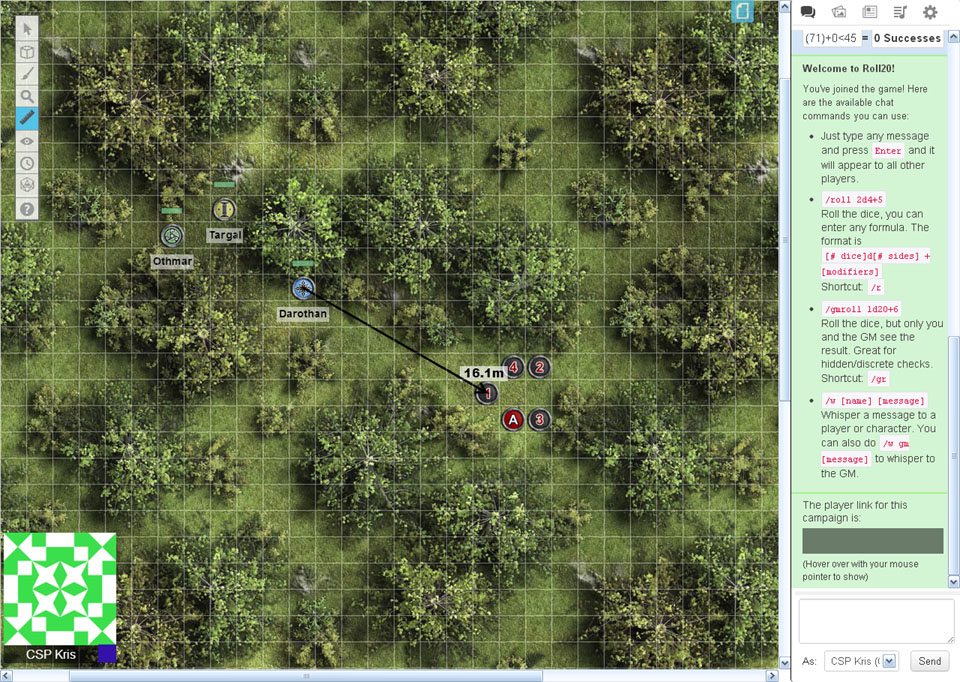
\includegraphics[width=0.75\linewidth]{roll20-example.jpg}
				\caption[Roll20 Screenshot]{A screenshot taken from the Roll20 web-app showing the table-top, text and voice chat functionality \citep{roll20-example}.} \label{fig:roll20}
			\end{figure}
		
			Roll20 \citep{roll20} was a popular web-app that was developed to enable games of \dnd \ to function without the need of a group of people coming together at a table. Instead, the group would use Voice over IP (VoIP) technologies (such as Skype or Roll20's internal VoIP system) to communicate and the Roll20 app would serve as the gaming table (see Figure \ref{fig:DnDLive}). 			
			
			Figure \ref{fig:roll20} shows a typical Roll20 virtual table-top in use. In comparison, we can see that the grid in the screenshot was very similar to the battle mat shown in Figure \ref{fig:DnDLive}. The DM of a group could use Roll20 to plan encounters and scenes for the party, and illustrate certain points to greater effect than at a physical table. All dice rolling could be performed from the Roll20 chat system, with graphical dice rolling across the virtual table-top. Without the Roll20 web-app, some groups would not be able to function. However, for other groups, the removal of the personal touch of meeting in person was not acceptable. 
					
			Roll20 was more than just a virtual table-top, as a quick reference database could be accessed through the purchase of \WotC \ books in a similar manner to \dnd \ Beyond (see Section \ref{sec:dnd-beyond}), as demonstrated in Figure \ref{fig:mm-purchases}. 
			
			\subsubsection{Kobold Fight Club} \label{sec:kfc}
			\begin{figure}
				\centering
				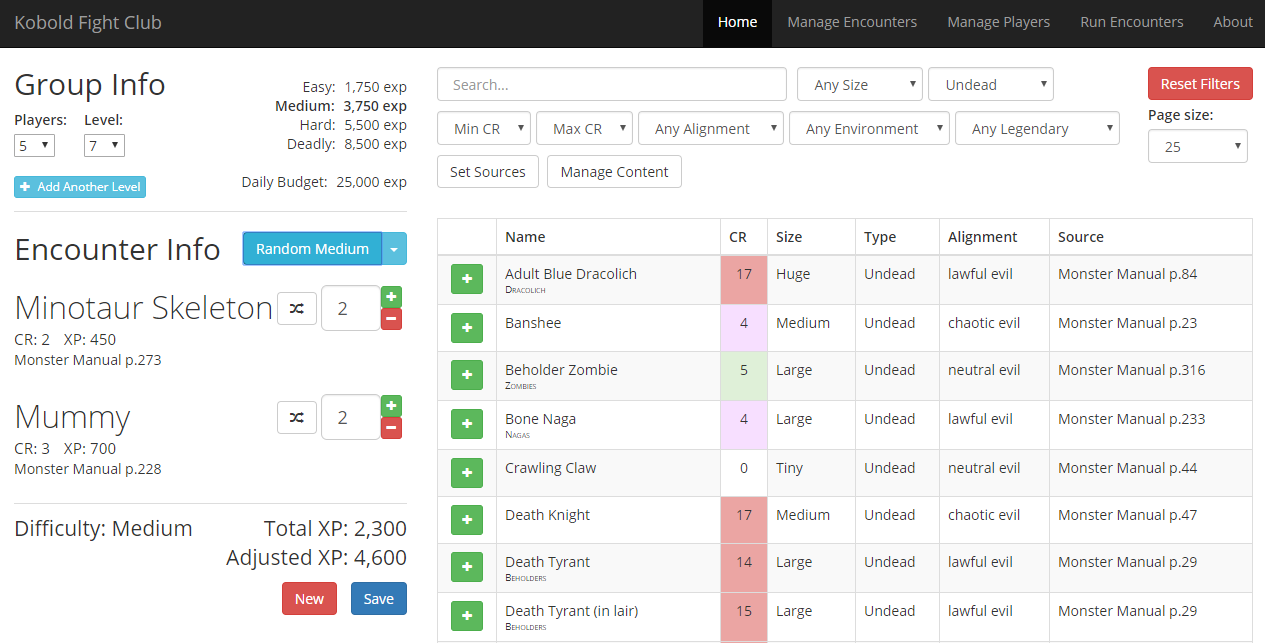
\includegraphics[width=0.8\linewidth]{kfc-screenshot.png}
				\caption[Kobold Fight Club Screenshot]{A screenshot showing an encounter designed using the Kobold Fight Club website, a popular \dnd \ encounter building tool}\label{fig:kfc}
			\end{figure}
			
			Kobold Fight Club (KFC) \citep{kfc-homepage}, named after one of the most popular monsters in \dnd, was a website that assisted many DMs in creating and balancing encounters with enemies during a campaign. KFC only had a single function at the time of writing, which was the encounter planning functionality. KFC was an example of a website that provided a single service to an excellent standard, with a clean User Interface (UI) that was easily understood, as shown in Figure \ref{fig:kfc}. KFC does have some weaknesses, in order to make the service free and open to all, the developers could not include the attributes of each monster. Instead, they can only provide a page reference so that the selected monsters could be found in the \WotC \ publications.
	
		\subsection{Software Engineering} \label{sec:software-eng}
		The \Codex \ project was not only the development of a web app based around the game of \dnd. It was the evaluation and examination of a single developer Software Engineering Agile methodology. In order to perform this evaluation, we must first gain an understanding of the Software Engineering Discipline (see Section \ref{sec:what-se}). From there we will learn about the Agile principles and observe the changes they brought to Software Engineering (see Section \ref{sec:what-agile}). Finally, we will examine two potential single developer agile methodologies, which would be compatible with the development of the \Codex \ web app (see Sections \ref{sec:agile-solo} and \ref{sec:xp-for-one}). 
			
			\subsubsection{What is Software Engineering?} \label{sec:what-se}
			As stated multiple times throughout this paper, \Codex \ was not only the development of the \Codex \ web app. The \Codex \ project aimed to evaluate a Software Engineering Agile methodology that was suited for the single developer. In this subsection, we will learn what Software Engineering was, at the time of writing, before gaining an understanding of the Agile Principles (see Section \ref{sec:what-agile}). 
			
			\begin{displayquote}
				"The systematic application of scientific and technical knowledge, methods and experience to the design, implementation, testing and documentation of software." -- \cite{SE-def}
			\end{displayquote}
		
			The above definition of Software Engineering explains that the discipline was the application of engineering practices to the development of Software, in order to produce the best Software solution to the proposed problem. These practices were reduced down to a series of stages that each project would be expected to progress through at least once during the project life cycle. Software Engineering was applied to a project through Software Engineering Methodologies (SEMs). Please note that these stages may have different names depending on the selected SEM, however generally they were known as:
			
			\begin{itemize}
				\item Requirements analysis
				\item System Design
				\item Implementation or Development
				\item Testing
				\item Deployment
				\item Maintenance				
			\end{itemize}
		
			\emph{Requirements analysis} (sometimes called requirements engineering) was when a developer (or team of developers) would discuss the problem with the client. The aim of this would be to create a well-defined list of requirements that a potential software system would need to fulfil to be a success. Later that list would be prioritised into four lists using a MoSCoW analysis (see Section \ref{sec:design} for the \Codex \ MoSCoW analysis). Those lists being Must Have, Should Have, Could Have and Won't Have. Several other investigative techniques may be used during the requirements analysis stage of a project, (sometimes referred to as \emph{Systems Analysis}) such as Rich Pictures and Stakeholder Wheels. By the end of a requirements analysis stage, the project would have a clear set of criteria that it has to meet in order to succeed.
			
			The \emph{System Design} stage was closely related to the requirements analysis stage and they were sometimes merged together by some methodologies. During this stage, the developers would design the proposed software system. This does not only mean the graphical look of the system; but the architecture that organises the classes, the methods that populate them and how information would be transferred between different parts of the system. This stage would produce a document known as the \emph{Design Document} (see Section \ref{sec:design}). This document would give future developers the information necessary to contribute towards the development of a system and would be regularly updated throughout each iteration of a project. The \Codex \ web app design document may be found within the supporting materials.
			
			During the \emph{implementation (or development)} stage of a project, the developers would build the system as designed from the previous stages. Depending on the SEM being used by the development team, there might have been the ability to revisit the requirements and design stages in order to fix unforeseen design errors or adjust to changing client demands. 
			
			The \emph{testing} stage of a project may occur during or after the implementation stage, depending on the applied SEM. Developers who practised \emph{Test Driven Development} (TDD) would have a large base of automated tests that would check a percentage of the code regularly \citep{TDD}. That percentage is known as \emph{code coverage}. Regardless of whether TDD was used during the implementation stage, the developers would still perform rigorous testing. This testing would involve the developers attempting to find bugs and/or security issues within the system. Eventually letting individuals (such as prospective users or experts in software security) test the system in order to gather feedback and different opinions on the current system. One such method of testing using these individuals might be a \emph{Think-Aloud Evaluation} \citep{thinkaloud}. Any issues found during this stage would be corrected by the developers before proceeding into the \textit{deployment} stage \citep{testing}.
			
			The \emph{deployment} stage of a system was a crucial moment in any project. Developers had several processes to choose from when deploying their system; direct, parallel, phased or piloted distribution. Each has their own strengths and weaknesses. Different systems would benefit the most from different deployment processes. 
			
			Once a system has been deployed, the maintenance stage may begin. Whilst during this stage additional features may be implemented into the system, they would fall into a life cycle of their own. Maintenance stage activities are limited to the identification and correction of any errors within the system, and it would have no definitive time scale. As long as the system was running, regular maintenance would have to be performed.
						
			\begin{figure}[h]
				\centering
				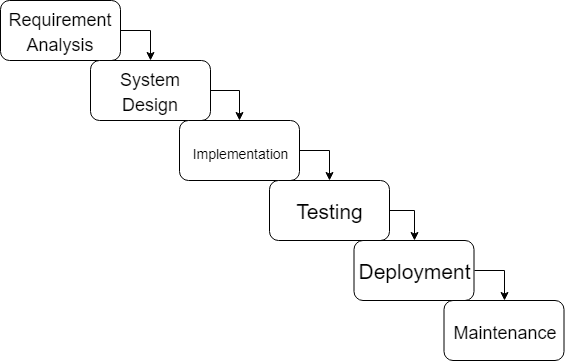
\includegraphics[width=0.8\linewidth]{waterfall.png}
				\caption[Waterfall Flow Diagram]{Flow Diagram showing the linear progression of a Waterfall Project.} \label{fig:waterfall}
			\end{figure}
			
			There was a variety of SEMs that have been tried and tested by several projects, with each possessing strengths and weaknesses. The earliest SEMs followed a \emph{Waterfall model}, where each stage would be completed in a linear sequence (see Figure \ref{fig:waterfall}). The popularity of Waterfall models arose from the simplicity they brought from a managerial point of view. The lack of iterations allowed a project manager to ``cross off" each section in sequence and move onto the succeeding tasks. The industry would eventually realise that the rigid linearity of the Waterfall model prevented the developers adapting to changing client demands. 
			
			\begin{figure}
				\centering
				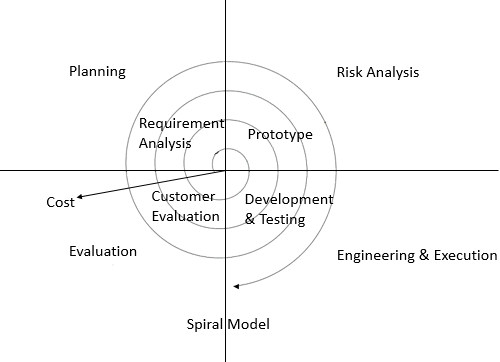
\includegraphics[width=0.8\linewidth]{spiral.png}
				\caption[Spiral Model Flow Diagram]{Flow Diagram showing the iterative design of the Spiral Model \citep{spiral-model-source}.} \label{fig:spiral}
			\end{figure}
			
			Iterative SEMs were created, such as the \emph{Spiral Model}, that formed the basis for the Agile Principles to be created (see section \ref{sec:what-agile}). The Spiral Model, as seen in Figure \ref{fig:spiral}, followed an iterative design that condenses the system life cycle into four distinct phases: planning, risk analysis, engineering \& execution and evaluation. Within the planning phase, the activities that were usually be associated with the requirements analysis and system design stages would be found. Risk analysis, an additional stage added by the Spiral Model, would ask the developer to prototype and examine the designed system. This was done in an attempt to reduce the number of errors that would need fixing further into the project, thus reducing costs. The engineering \& evaluation stage would see the approved system built and tested, before finally deploying just prior to the evaluation stage, where the users would provide feedback. That feedback was then incorporated into the next iteration of the project, where the spiral would begin anew.
			
			The \Codex \ web app development has followed a methodology, discussed in Section \ref{sec:agile-solo} and was described as a Software Engineering project. This means that the development followed the systematic application of engineering practices, managed by the Agile Solo methodology.
				
			\subsubsection{What is Agile?} \label{sec:what-agile}
			Agile was a set of ideas and principles that would change the way in which software was developed. The creators of Agile were frustrated with how software were being built in the 1980s and 90s. Before Agile, a linear approach was taken (see Figure \ref{fig:waterfall}) towards software development. For example, once a set of requirements for a system was decided, it could not be changed because the project methodology would not allow it. One of the frustrations were lengthy and complicated contracts that bound both client and developers to a proposed system. These frustrations drove the creators of Agile, who wanted to ``\ldots uncover better ways of developing software \ldots" to create the \textit{Agile Manifesto}, which at its core contained 4 values \citep{AgileManifesto}:
			
			\begin{enumerate}
				\item \textbf{Individuals and interactions} over processes and tools
				\item \textbf{Working software} over comprehensive documentation
				\item \textbf{Customer collaboration} over contract negotiation
				\item \textbf{Responding to change} over following a plan 
			\end{enumerate}
		
			The Agile Manifesto additionally states ``\ldots while there is value in the items on the right, we value the items on the left more". This distinction is critical to Agile, as the creators recognised that the traditional Software Engineering methods held a value. However, change must be embraced in order to keep up with the demands of the future.
			
			With the release of the Agile Manifesto, many iterative SEMs became more popular and replaced the linear waterfall models as the industry standards. Scrum and Kanban are two such SEMs. 
			
			The Scrum methodology was governed by a ``\ldots simple set of roles, responsibilities and meetings that never change" \citep{scrum-online}. The roles within a scrum team are \emph{Product Owner}, \emph{Scrum Master} and \emph{Team}. The Product Owner may be a client or an executive who guides the Scrum Master and the Team towards creating the product that should be delivered. Technical expertise was not required and the Product Owner should not be involved in the management of the development process. The Scrum Master was the facilitator towards both the Team and Product Owner, meaning that this individual would remove any impediments preventing the progress of the project. Scrum Masters do not manage the Team however as the Team is entirely self-managing. Scrum Teams would comprise of three to six members, who would select the work to do every \emph{sprint} in a \emph{sprint planning meeting}. Teams would contain a mixture of professionals including but not limited to software engineers, architects and User Interface (UI) designers \citep{Scrum}. 
			
			\begin{figure}
				\centering
				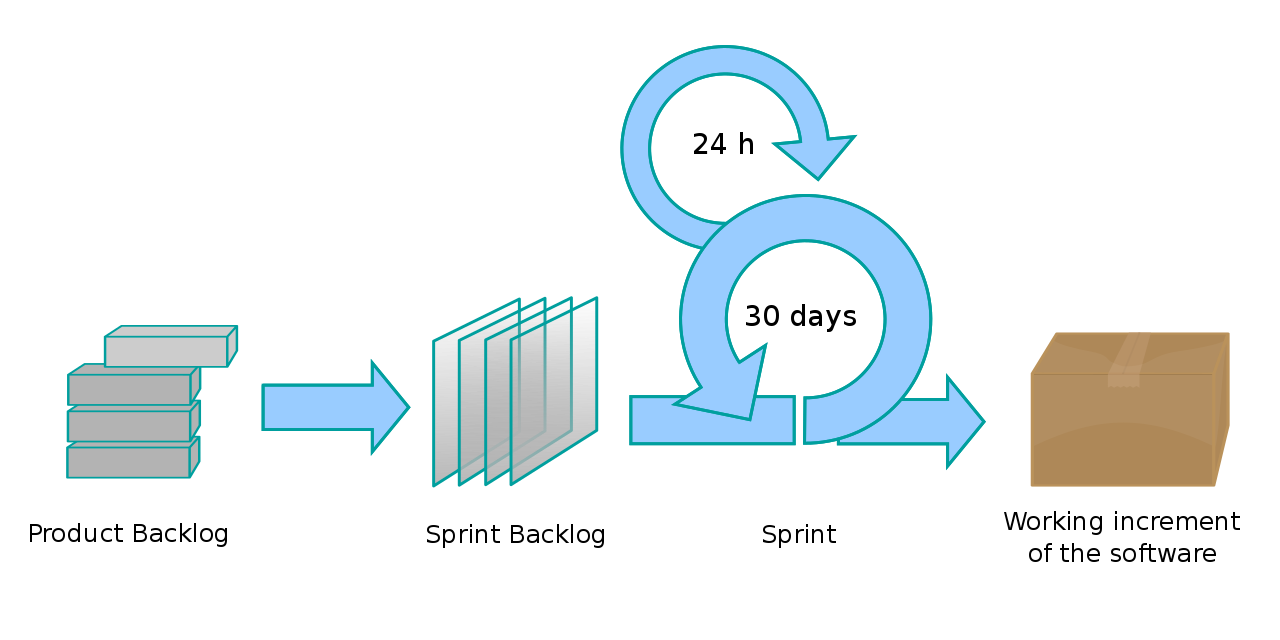
\includegraphics[width=0.8\linewidth]{scrum.png}
				\caption[Scrum Methodology Sprint Cycle]{Flow diagram detailing the stages of a Scrum \emph{sprint} cycle. At the beginning of each \emph{sprint} the Team and Scrum Master would select a set of tasks from the \emph{Product Backlog} and move them into the \emph{Sprint Backlog}. This occurs during the \emph{Sprint Planning Meeting}. During the two to four week \emph{sprint} the Team would progress through the \emph{Sprint Backlog} tasks, holding a tightly regulated short \emph{Scrum Meeting} daily. At the end of the \emph{sprint} the Team would have produced a potentially shippable increment of working software.} \label{fig:scrum}
			\end{figure}
		
			Scrum projects were organised into \emph{sprints}. At the beginning of each \emph{sprint} the Team and Scrum Master would select a set of tasks from the \emph{Product Backlog} and move them into the \emph{Sprint Backlog}. This occurs during the \emph{Sprint Planning Meeting}. During the two to four week \emph{sprint} the Team would progress through the \emph{Sprint Backlog} tasks, holding a tightly regulated short \emph{Scrum Meeting} daily. This meeting would last for approximately five minutes and was hosted by the Scrum Master. Scrum Meetings served as a platform for each Team member to declare what work was done during the previous day, the work to be done today and any impediments preventing the work from being achieved. At the end of the \emph{sprint} the Team would have produced a potentially shippable increment of working software. This increment would be scrutinised in the \emph{Sprint Retrospective Meeting} which evaluated the work done, and any large-scale issues would be solved before beginning the sprint anew with another \emph{Sprint Planning Meeting}.
			
			Whilst some projects would only use Scrum during the implementation stage of a project, perhaps within an iterative Spiral model (see Section \ref{sec:what-se} and Figure \ref{fig:spiral}), other projects would choose to use Scrum throughout the project life cycle to prevent confusion through the use of multiple different SEMs. 
			
			\begin{figure}
				\centering
				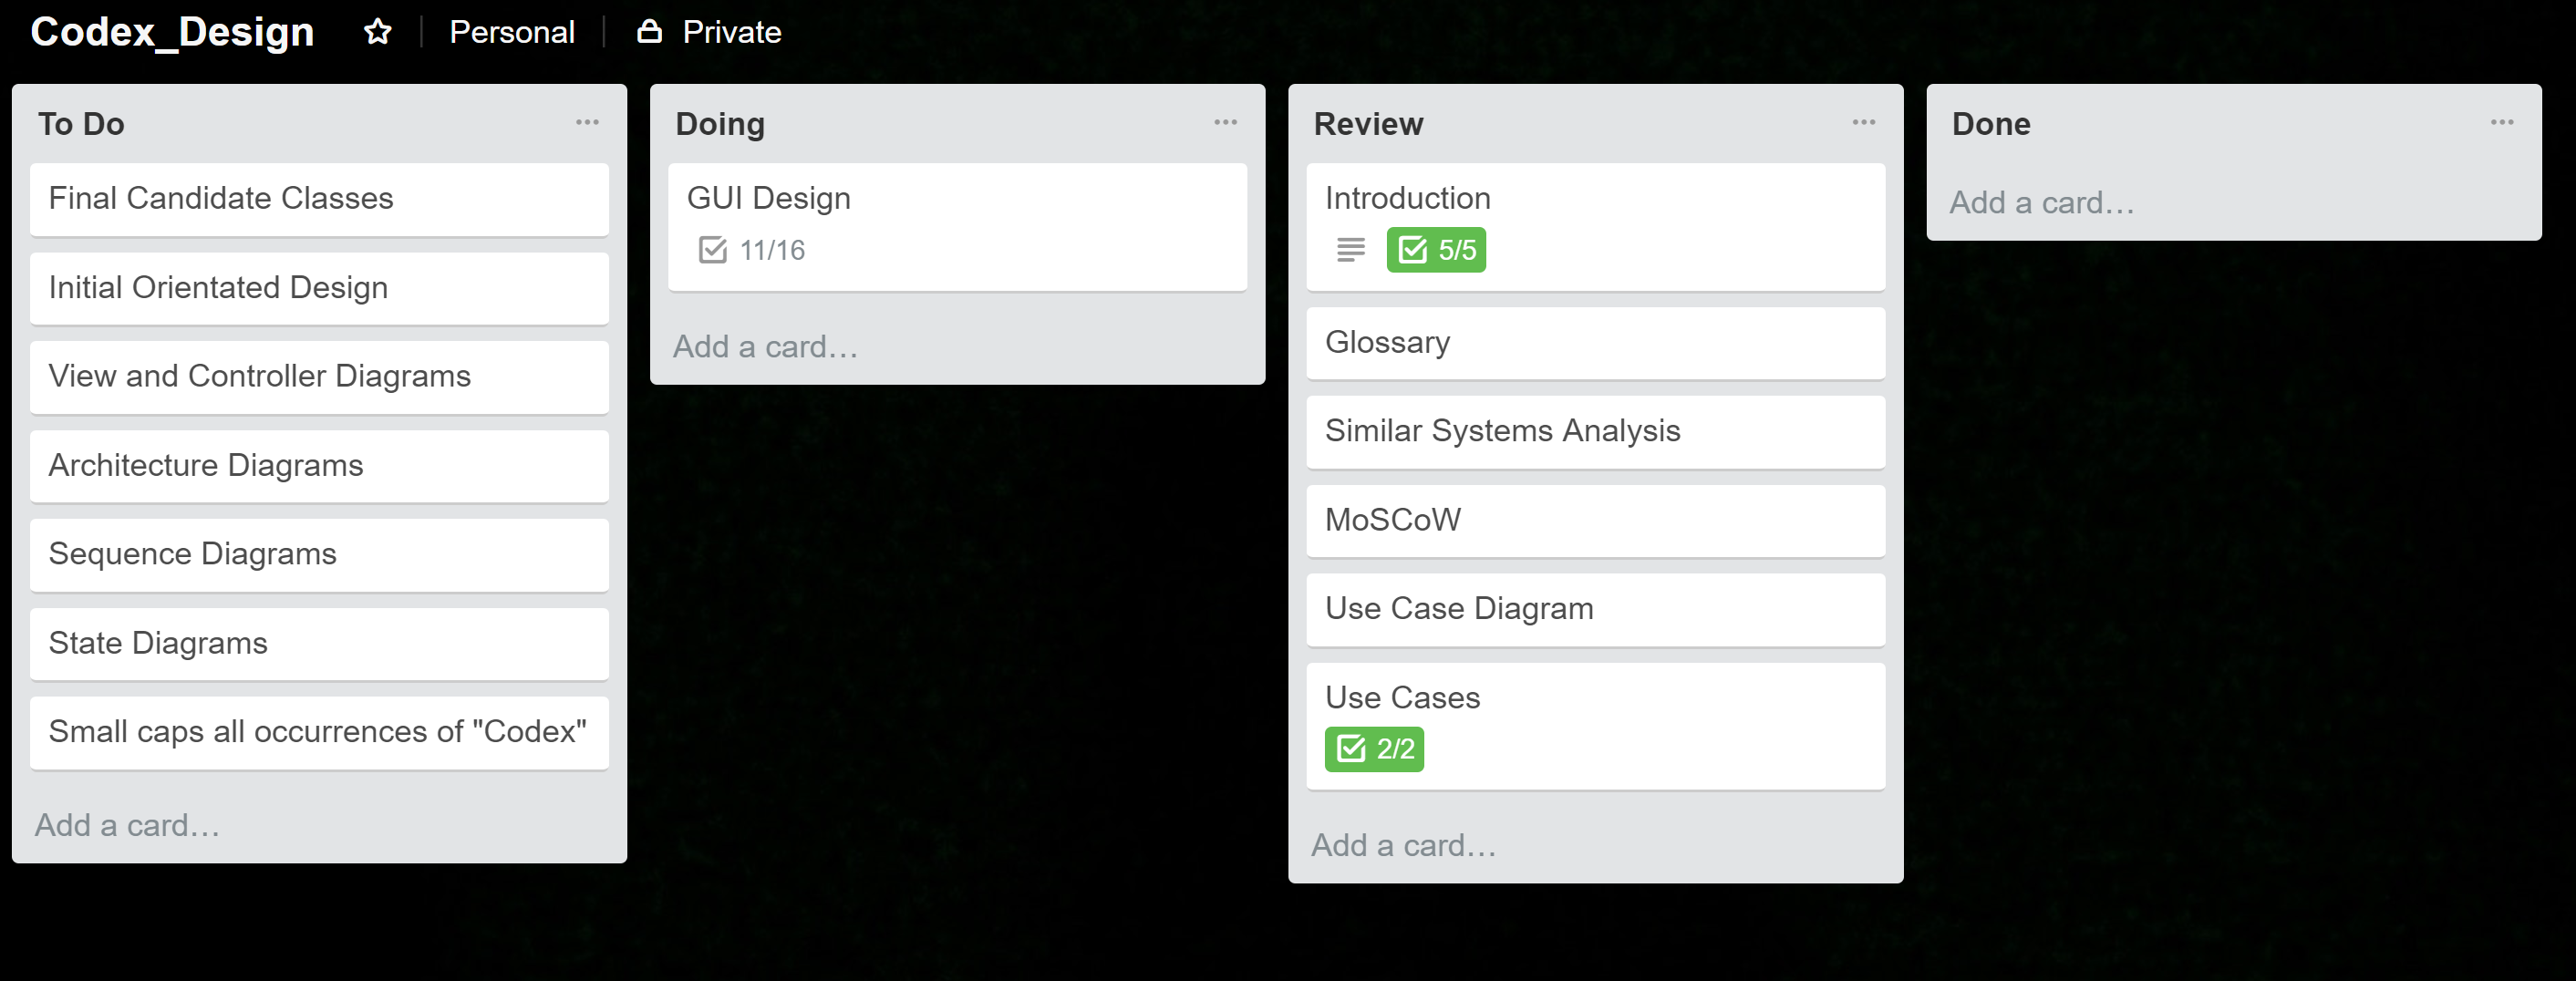
\includegraphics[width=0.8\linewidth]{trello_board.png}
				\caption[Example Kanban Board using Trello]{Screenshot taken from the early design stage of the \Codex \ web app. Kanban Board developed using the Trello app \citep{trello} and includes an optional Review column.} \label{fig:kanban}
			\end{figure}
		
			Kanban was another popular Agile SEM, which whilst closely related to Scrum was a lean methodology rather than iterative. Despite this difference, Kanban was often used in conjunction with iterative SEMs, the most common being Scrum \citep{kanban}. Kanban was operated by balancing the demands of a project with the available capacity of the development team, with the ultimate goal of reducing the effect of system-level bottlenecks. This was achieved through the use of a Kanban Board (see Figure \ref{fig:kanban}), which may have been either physical or digital. Kanban board must include the following columns: \emph{to do} (sometimes called Backlog), \emph{Doing} and \emph{Done} at a minimum. However, additional columns such as; \emph{plan}, \emph{test} (or review) and \emph{deploy} were recommended. The task \emph{tickets} would move from left to right through each of the columns on the board, eventually clearing the Backlog of tasks. Some users of Kanban might have colour coded tickets in accordance with the different type of tasks; pink for development tasks and yellow for design tasks for example. Customisation of the tickets can be taken further when developers apply arbitrary levels of difficulty to the tickets in order to gauge the length of time taken to complete that task. 
			
			Kanban projects would not have to go through the regular planning that Scrum projects experiences, because Kanban projects were not organised into Sprints. However, Scrum can benefit from the inclusion of Kanban boards to organise and manage the Product and Sprint backlogs.
			
			\subsubsection{Agile Solo} \label{sec:agile-solo}
			Agile Solo was an SEM developed by Anna Nystr{\"o}m in June 2011 \citep{AgileSolo}. The methodology was created using the values stated by the Agile Manifesto (see Section \ref{sec:what-agile}) and aimed to adapt the established working practices of existing Agile SEMs. However, the definitive feature of Agile Solo is that the methodology was able to be implemented and used by a single developer. 
			
			Nystr{\"o}m selected the suitable components from many different existing Agile SEMs, such as the Sprint Cycle from Scrum (see Figure \ref{fig:scrum}) and the Kanban Board (see Figure \ref{fig:kanban}) from Kanban to name but a few. However, Nystr{\"o}m also realised that single developers rarely work in isolation as typically there would be a supervising individual assigned to the project and a client who would own the project, so adaptations were made to accommodate such individuals.
			
			\begin{figure}[H]
				\centering
				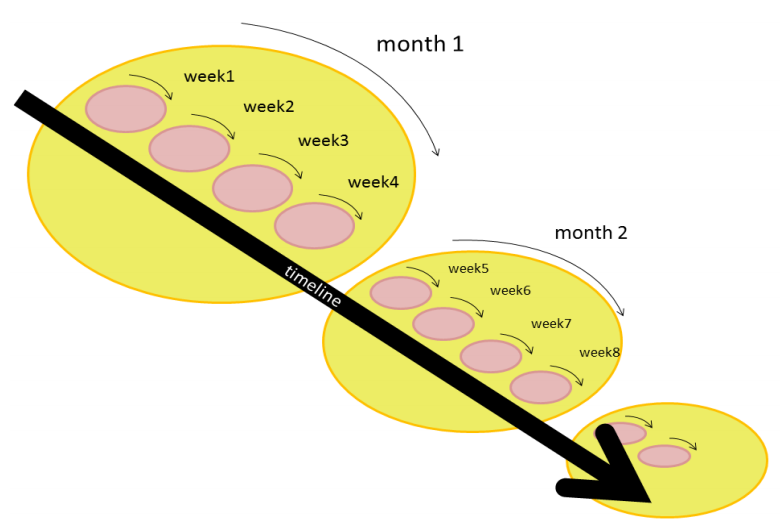
\includegraphics[width=0.8\linewidth]{agile-solo.png}
				\caption[Agile Solo Diagram]{Diagram to represent the Agile Solo Software Engineering Methodology. The project is segmented into \emph{Monthly Cycles} that would contain \emph{Weekly Sprints}. The developer would review the work done at the end of each Sprint, with the customer and supervisors reviewing the work at the end of each cycle. The Monthly Cycle would begin anew with feedback from the customer and supervisor to be incorporated into the project \citep{AgileSolo}.} \label{fig:agile-solo}
			\end{figure}
			
			The resulting methodology was called Agile Solo and revolved around monthly cycles with weekly Sprint iterations. At the end of every Sprint the developer would review and test the work done, whilst at the end of each cycle the customer and supervising figures would review and test the system providing feedback to be incorporated in the next cycle. This is demonstrated by Figure \ref{fig:agile-solo}. Nystr{\"o}m recommends that the product backlog should be managed by a Kanban Board and the software be implemented using Test Driven Development (TDD). 
			
			Agile Solo was selected to be the SEM for the development of the \Codex \ web app (see Section \ref{sec:use-agile-solo}), and shall be evaluated later in this paper (see Sections \ref{sec:agile-solo-effect} and \ref{sec:agile-solo-eval})
			
			\subsubsection{XP for One} \label{sec:xp-for-one}
			Extreme Programming (XP) was an SEM which would attempt to improve the software quality through an iterative development loop that emphasised responsiveness to changing customer requirements. Typically paired with programming practices such as TDD and pairs programming, practitioners of XP believed that the only important product of development was code \citep{XP}.  
			
			\begin{figure}[H]
				\centering
				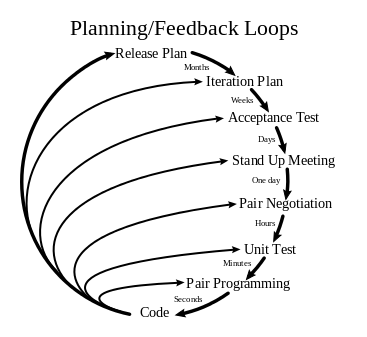
\includegraphics[width=0.6\linewidth]{xp.png}
				\caption[Extreme Programming Diagram]{Diagram to represent the Extreme Programming iterative life cycle \citep{xp-diag}.} \label{fig:xp}
			\end{figure}
			
			As seen in Figure \ref{fig:xp}, XP was highly iterative, with each task within the SEM having an iteration cycle. XP for One was an untested development methodology which had one critical difference from traditional XP, the removal of Pair Programming (pair negotiation in the diagram) \citep{SoloXP}. 
			
			In the event that Agile Solo (see Section \ref{sec:agile-solo}) was discovered to be unsuitable towards the development of the \Codex \ web app, XP for One was to be the replacement SEM.
			
		\subsection{Web App Technology} \label{sec:web-app}
		The \Codex \ web app was designed to be a Web Application (web app). In this Section, we will learn what a web app was and how it differed from the traditional websites and applications (see Section \ref{sec:what-web-app}). ReactJS was a popular library for the JavaScript programming language that was developed specifically to develop User Interfaces (UI). Due to the popularity and availability of supplementary materials of ReactJS, it was selected to developer the \textit{front-end}\footnote{The front-end back-end split was a common phrase when distinguishing what components of the system a user could see, and what they could not see. Front-end reflects the Graphical User Interface (GUI) for the system, whilst the Back-end will contain the Server and Database components of the system.} of  the \Codex \ web app (see Section \ref{sec:react-js}). Finally, we will explore the server and database (\textit{back-end}) that supports the \Codex \ web app, built in \textit{Node.js} and \textit{MySQL} (see Section \ref{sec:backend}). Before quickly examining how the front-end and back-end of the system will communicate with each other in what was known as the \emph{stack} (see Section \ref{sec:stack}).
		
			\subsubsection{What is a Web App?} \label{sec:what-web-app}
			With the rising popularity of applications in the early 2000s, web developers understood the need to reinvigorate websites with new technologies to bring websites into the modern age. This resulted in the creation of web apps; a system that could operate as a separate application on a computer or mobile device, that could still be accessed through a browser (such as Google Chrome). Today web apps exist in between applications and websites \citep{web-apps}. 
			
			\begin{figure}[h]
				\centering
				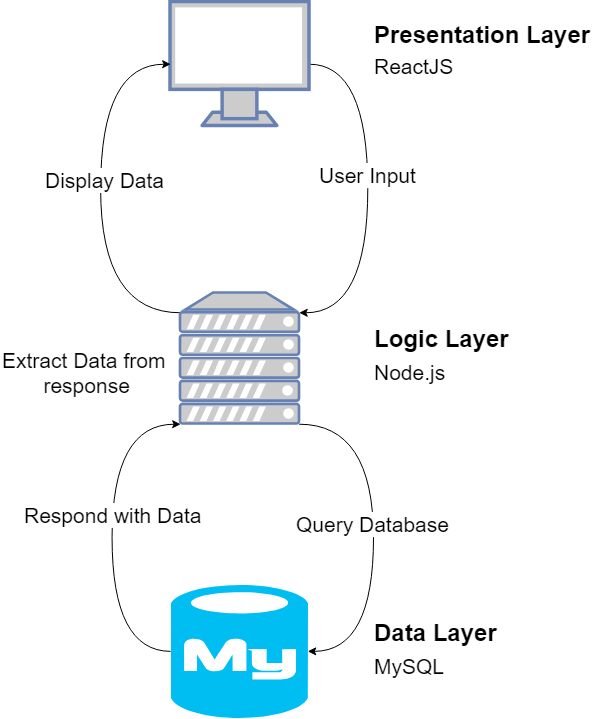
\includegraphics[width=0.5\textwidth]{web-app-arch.PNG}
				\caption[Three Tiered Web App Architecture]{Diagram showing the flow of information between the three tiers of web app architecture. The \emph{presentation layer} allowed the user to interact with the system (and vice versa). The \emph{logic layer} would host the functionality of the system and generated the GUI. Finally the \emph{data tier} would hold the database that supported the web app.} \label{fig:web-apps}
			\end{figure}
		
			The \Codex \ web app will follow the web app three-tiered architecture that was established with the technologies emergence. As we can see from Figure \ref{fig:web-apps} the first layer (Presentation Tier) was held locally on the Client's machine. Known as the `Client-Side'. Here HTML, CSS and JavaScript were used to translate data into a format the Client will understand. In the second layer (Logic Tier), languages such as ReactJS perform functions on raw data to generate web content. Traditionally the Logic Tier was hosted on a Server that Clients connect to, this is the `Server-Side' The third layer (Data Tier) communicates with the Logic Tier through SQL Queries \citep{SecurityWebApps}. 
			
			\subsubsection{ReactJS} \label{sec:react-js}
			ReactJS was a JavaScript library developed by Facebook, Inc. after the acquisition of Instagram \citep{ReactJSOfficial}. The library provided a set of components, and the ability for developers to create custom components, that would be rendered by the VirtualDOM (explained in Section \ref{sec:codex-development}). This allowed developers to quickly build user interfaces that were highly customisable without the use of traditional HTML components \citep{MasteringReact}. The supporting language for ReactJS was JavaScript, which allowed the use of many custom, open-source packages to further improve the ReactJS library.  
			
			Due to the popularity, at the time of writing, that ReactJS held within the Industry \citep{ReactJSPopularity}, the developer chose to use ReactJS to developer the UI and Navigation elements of the \Codex \ web app system. This would be later paired with the Node.js Server and MySQL Database to form the \emph{stack} (see Section \ref{sec:stack}).
			
			\subsubsection{Node.js Servers and MySQL Databases} \label{sec:backend}
			Node.js was an asynchronous event driven by the JavaScript runtime that was developed to build scalable network applications (commonly known as Servers) \citep{nodejsOfficial}. In the context of the \Codex \ web app, this server would be ran locally during development (specifically Port 4000), but could be later migrated to a dedicated URL. The role of the \Codex \ server would be act as the communication method between the ReactJS application (hosted on Port 3000) and the MySQL Database. Variables would be passed to the database by including variables in the URL that were later extracted by Node.js into SQL queries before passing that query to the Database. The result would be transferred back to the ReactJS front-end via the response function of Node.js.
			
			\begin{lstlisting}[caption={Node.js source code which was used to connect the Node.js Sever to the MySQL Database, forming the back-end of the application.}, label={cod:db-connect}]
			const mysql = require('mysql');
			const connection = mysql.createConnection({
				host	: 'localhost',
				user	: '<username>',
				password: '<password>',
				database: 'codex'	
			});
			connection.connect(err => {
				if(err) {
					return err;
				} else {
					return console.log('connected')
				}
			});
			\end{lstlisting}
			
			The MySQL Database was populated with test data and connected to the Node.js server using the \emph{mysql} JavaScript package, an example of which can be seen in Listing \ref{cod:db-connect}. The developer told the JavaScript runtime compiler that it would require the \textit{mysql} package in order to then use the \texttt{createConnection()} method (line 2) to store the authentication details for the Database. Finally, the server would use the authentication details to connect to the database and test the connection on line 8.
			
			\subsubsection{ReactJS/NodeJS/MySQL Stack} \label{sec:stack}
			The ReactJS front-end (see Section \ref{sec:react-js}) and the Node.js back-end (see Section \ref{sec:backend}) ran on ports 3000 and 4000 respectively. When the two halves of the application would function together they would be referred to as the \emph{Stack}, and mirrored the Web App Architecture diagram (see Figure \ref{fig:web-apps}). 
			
	\section{Development and Implementation} \label{sec:dev-and-imp}
	In this Section we will examine how the Agile Solo methodology (discussed in Section \ref{sec:agile-solo}) will be implemented into the \Codex \ project and later evaluated in Sections \ref{sec:agile-solo-effect} and \ref{sec:agile-solo-eval}. Next, we will gain an understanding of the design of the \Codex \ web app through the extensive Design Document that can be found in the supporting materials. Finally, we will expand upon the knowledge gained in Sections \ref{sec:react-js} and \ref{sec:backend} to gain an appreciation for the development of the \Codex \ web app by dissecting some examples of source code.
	
		\subsection{Using Agile Solo} \label{sec:use-agile-solo}
		As explained in Section \ref{sec:agile-solo}, Agile Solo was centred around the idea of \textit{weekly sprints} encompassed by \textit{monthly cycles} (see Figure \ref{fig:agile-solo}. Whilst there was no recommendation by Nystr{\"o}m for the management of the project backlog, the \Codex \ implementation of Agile Solo will utilise the Product Backlog/Scrum Backlog system favoured by Scrum (see Section \ref{sec:what-agile}). At the end of each sprint, the developer (the author of this paper) would test the \Codex \ system as it stood, in order to catch any issues that surpassed the automated tests. A fortnightly meeting would be held with the supervisor of the project in order to ensure that the development of \Codex \ remained on track. At the end of each cycle, the current state of the \Codex \ web app would be presented to a small group of users in order to ascertain the quality of the development done.
		
		The feedback generated from the supervisor and user meetings was stored within the project journal (found in the supporting material) and was later incorporated into future developments, where possible. Also found in the journal, would be the initial evaluations and opinions of Agile Solo from the developer as the development of the \Codex \ web app progressed. 
		
		\subsection{Design} \label{sec:design}
		The \Codex \ web app was designed through the creation of a Design Document \footnote{The \Codex \ Design Document can be found in the supporting material for this paper.}, which was briefly discussed in Section \ref{sec:what-se}. There we learned that a Design Document should contain a mixture of diagrams and analysis in order to convey to a new developer the design of a software system \citep{DesignDocExample}.
		
		These would include the analysis of requirements and similar systems. These analyses would produce diagrams to explain how the system was intended to be used, the GUI design, Class and Architecture Designs. Additional diagrams may be included to illustrate the flow of information throughout select use cases.
		
		The requirements analysis would consist of listing, in detail, the primary functions of the system. The \Codex \ Design Document elected to use bullet points in order to promote concise descriptions of the functionality. Bullet points additionally allowed the developer to highlight certain functions as sub-functions. For example; the ``Account Creation" functionality possessed the sub-function that there should be ``Two `levels' of accounts - Player and Dungeon Master" within the system. From this detailed list, a \emph{MoSCoW analysis} can be performed. The developer would designate which functions were critical to the success of the system and which functions would not be critical. MoSCoW contains four categories of functionality; Must Have, Should Have, Could Have and Won't Have. The \Codex \ web app MoSCoW analysis can be found within the Design Document in the supporting materials.
		
		The \emph{Similar System} analysis was a vital step for Design Documents, particularly for the \Codex \ web app, as it would ensure that the developer was not creating a duplicate for a system that already existed. Therefore, for commercial systems, this analysis may be seen as a form of risk assessment. Typically the findings of the Similar Systems analysis are stored within a table in the early stages of the Design Document. Sections \ref{sec:dnd-beyond}, \ref{sec:roll20} and \ref{sec:kfc} informed by the findings from the \Codex \ Similar Systems analysis. 
		
		Another key component of a Design Document would be the \emph{Glossary of Terms}, which would inform future developers of the terms required to understand the software system. The terms contained within this glossary would not extend to technical terms unless they were uncommon at the time of development. Instead, the glossary would focus on the contextual terms, in the case of \Codex, the majority of the terms were \dnd \ related. The full glossary of terms for the \Codex \ web app can be found in the Design Document.
		
		For every function detailed by the Design Document, there would be an accompanying \emph{Textual Use Case} and \emph{Use Case Table} which were then summarised into a \emph{Use Case Diagram}. The Use Case Diagram would show the authorisation that each type of user would have within the system. In the case of \Codex, we have two types of users -- players and DMs -- and each had two levels of access to the system functions. Also shown by the Use Case Diagram is which use cases relationships: \emph{include} (meaning they are a prerequisite to) and \emph{extends} (which represents optional behaviours between use cases). The textual use cases and use case tables detail exactly how each function of the app would be used by the user. These details included goals, scope, triggers, end conditions, success and alternative scenarios to name but a few. The developer would study the use cases in order to gain an understanding of what the source code needs to reflect prior to starting development.

		The Graphical User Interface (GUI) design of the \Codex \ web app began with \emph{lo-fi prototyping}, where the developer would roughly sketch the design of the GUI and then quickly receive feedback from prospective users. With the feedback incorporated into the design, the lo-fi prototypes were transformed into \emph{hi-fi prototypes} by creating digital sketches using the software. The \Codex \ web app GUI was designed using MarvelApp \citep{marvelapp}, which had a range of tools and allowed the prototyping of colour schemes and icons to be effectively tested. The hi-fi prototypes were shown to prospective users to gather feedback, who reported that the colour scheme was too dark \citep{GUIDesign}. With the lighter palette integrated into the app, the GUI design was finalised and inserted into the Design Document as images. 
		
		Once the use cases and functionality of a system had been decided, the developer could now start allocating the functionality to classes within the source code. This was done through the Class Diagram, which shows the flow of information between the classes that divide the source code. Each class within the diagram would have the class and method names. The method names were designed to be self-explanatory to the developer. This was done so that when the developer was writing the source code, the Class Diagram could be referenced so that development would stay on track and the scope of the project would not creep \footnote{\emph{Scope Creep} is a term used by Software Engineers when the Scope (the functionality) of a system was extending (creeping) past the original parameters of the system in an unplanned fashion.}.
		
		The classes generated from the Class Diagram would be inserted into the Architecture Diagram, to create a graphical representation of the system architecture. Each class was allocated into one of the three tiers of the web app architecture (described in Section \ref{sec:web-app} and Figure \ref{fig:web-apps}): Presentation, Logic and Data. Similar to the Class Diagram, the Architecture Diagram guided the developer during the development process to ensure that each class was performing the tasks allocated during the design process. 
		
		\subsection{Development of \Codex} \label{sec:codex-development}
		The development of the \Codex web app was scheduled to take nine weeks (see Figure \ref{gantt:pplan}), which allowed for multiple revisions of the design and development in addition to the writing and evaluation necessary for the project. 
		
		As mentioned in Section \ref{sec:web-app}, the \Codex \ web app was built using ReactJS (see Section \ref{sec:react-js}) supported by a Node.js and MySQL back-end (see Sections \ref{sec:backend} and \ref{sec:stack}). Before providing examples of the \Codex \ source code, we must first expand upon our understanding of how ReactJS operated.
		
		ReactJS was operated through the concept of \emph{components}. Developers would create these components, which would render the GUI within the logic layer before sending the view across to the presentation layer. Components could receive inputs from other components and from the database through the \emph{props} list. However, components may also be functional, not just presentational. Finally, ReactJS passes information across web pages through an attribute known as \emph{state}, components may be \emph{stateful} or \emph{stateless.}
		
		\begin{lstlisting}[caption={ReactJS source code which generated the GUI for the homepage for the \Codex \ web app}, label={cod:homepage}]
		class App extends Component {
			state = {
				users: [],
				user: {
					id: 0,
					name: '',
					password: ''
				}
			}
		componentDidMount() {
			this.loginUser();
		}
		loginUser = _ => {
			const { user } = this.state;
			fetch(`http://localhost:4000/user-login?name=${user.name}&password=${user.password}`)
				.then(response => response.json())
				.then(parsedJSON => parsedJSON.results.map(account => (
					{
						id: `${account.UserID}`
					}
				)))
				.then(users => this.setState({
					users
				}))
				.then(this.redirectToLanding)
				.catch(error => console.log('login failed', error))
		}
		redirectToLanding = _ => {
			const { user } = this.state;
			<Link to={`/dungeon-master?id=${user.id}`}/>
		}
		render() {
		const { user } = this.state;
		return (
			<div className="page-container">
				<img alt="Background" className="bg-img" src={background}/>
				<div className="header">
					<div className="login-container">
						<Segment padded>
							<Header as='h1' className="app-title">Welcome, Dungeon Master, to your Codex!</Header>
							<Input fluid placeholder="Username" type="text" onChange={e => this.setState({ user: { ...user, name: e.target.value }})}/>
							<Divider hidden/>
							<Input fluid placeholder="Password" type="password" onChange={e => this.setState({ user: { ...user, password: e.target.value }})}/>
							<Grid columns={2} relaxed>
								<Grid.Column>
									<Segment basic>
										<Button primary fluid onClick={this.loginUser}>Login</Button>
									</Segment>
								</Grid.Column>
								<Grid.Column>
									<Segment basic>
										<Link to={'/player'}><Button primary fluid>Reset Password</Button></Link>
									</Segment>
								</Grid.Column>
							</Grid>
							<Divider horizontal>Or</Divider>
							<Link to={'/create-account'}><Button secondary fluid>Sign Up Now</Button></Link>
						</Segment>
					</div>
				</div>
			</div>
		);
		export default App;
		\end{lstlisting}
		
		Listing \ref{cod:homepage} was the source code that generated the homepage of the \Codex \ web app (shown in Figure \ref{fig:homepage}) once compiled through the \emph{virtual DOM}\footnote{A \emph{virtual DOM} (Document Object Model) would behave in the same manner as the \emph{actual DOM}. Which would construct a node tree that lists all elements and corresponding attributes on a webpage. The difference was that the virtual DOM was significantly faster.}. The file would compile in the order we would read it. Within this example we can see the state of \texttt{App Component} being updated several times, both through user input via the \texttt{Input} fields on lines [] and [] or the results fetched from the \texttt{loginUser} method fetch statement. The ReactJS component method \texttt{componentDidMount()} was used to immediately update the state of the component, which would hold the data for the app. The source code used to extract the User Information from the URL shown on Line 11 can be found below in Listing \ref{cod:server-query}
		
		\begin{lstlisting}[caption={Source code for querying the Database with User Information}, label={cod:server-query}]
		app.get('/user-login', (request, response) => {
			const { name, password } = req.query;
			connection.query(`SELECT UserID FROM users WHERE UserName="${name}" AND UserPassword="${password}";`, (error, rows, results) => {
				if (error) {
					return res.send(error)
				} else {
					return res.json({
						data: rows
					})
				}
			});
		});
		\end{lstlisting}
		
		\begin{figure}
			\centering
			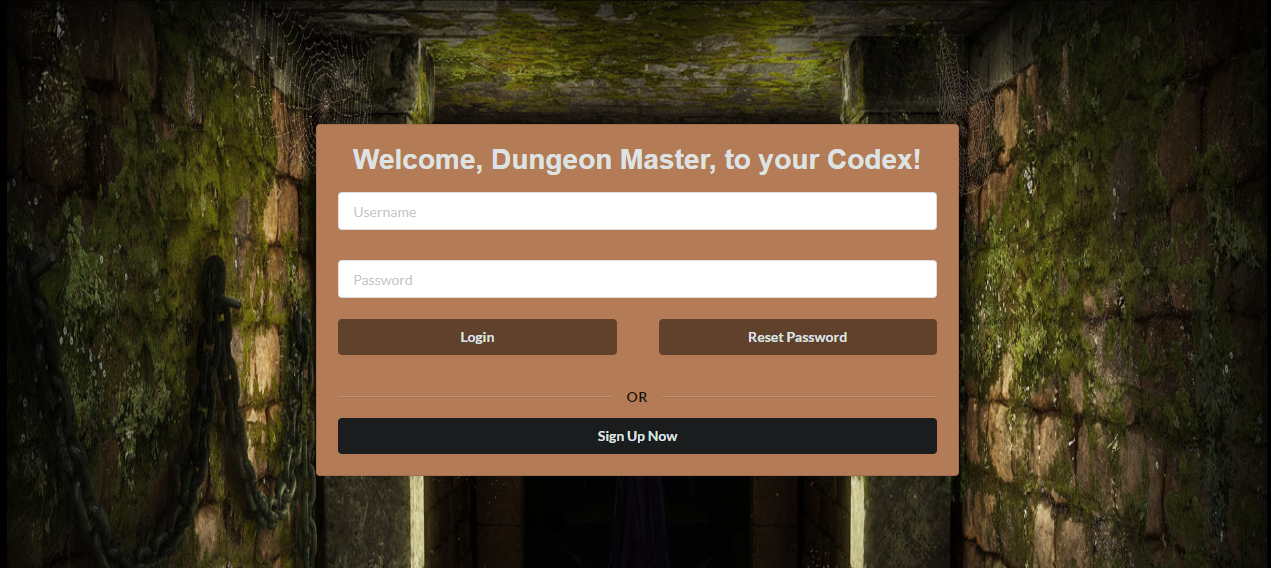
\includegraphics[width=0.8\linewidth]{homepage-developed.png}
			\caption[Screenshot of the \Codex \ web app]{Screenshot taken from the \Codex \ web app homepage which shows the rendered components detailed in Listing \ref{cod:homepage}} \label{fig:homepage}
		\end{figure}
	
		The development of \Codex \ was driven by tests, using the Test Driven Development (TDD) principle, in that each method will produce a testable outcome. Before any development could begin, the developer wrote a test that would ensure no build of the \Codex \ web app would be deployed when the components where unable to be rendered. This was known as a \emph{smoke test} which has been an industry standard test to include in an automated testing environment for over a decade \citep{testing}. Listing \ref{cod:smoke-test} was the source code that was necessary to perform the smoke test on the \Codex \ web app. When a build of the web app was pushed to the master build on GitHub \citep{github}, the code was automatically tested by the web service \emph{CodeShip} \citep{codeship} which would execute the \texttt{App.test.js} file before committing the changes to GitHub. As previously mentioned in Section \ref{sec:agile-solo}, TDD does not prevent every bug from infecting the master version of a project, but would prevent the majority of the developer errors increasing the quality of the code produced.
		
		\begin{lstlisting}[caption={\Codex \ web app smoke test}, label={cod:smoke-test}]
		import React from 'react';
		import ReactDOM from 'react-dom';
		import App from './App';
		
		it('renders without crashing', () => {
			const div = document.createElement('div');
			ReactDOM.render(<App />, div);
			ReactDOM.unmountComponentAtNode(div);
		});
		\end{lstlisting}
	
	
	\section{Outcome of the \Codex \ project} \label{sec:outcomes}
	In this Section we will examine the development of the \Codex \ web app (see Section \ref{sec:dev-obs} and the effectiveness of Agile Solo in managing the development (see Section \ref{sec:agile-solo-effect}). At the end of this section, we will have an understanding of the outcomes of the \Codex \ project and will then be able to evaluate those outcomes in Section \ref{sec:evaluation}.
	
		\subsection{Development Observations} \label{sec:dev-obs}
		The \Codex \ web app was developed in ReactJS (see Section \ref{sec:react-js}) using the Software Engineering Methodology (see Section \ref{sec:what-se}) known as Agile Solo (see Sections \ref{sec:agile-solo} and \ref{sec:use-agile-solo}). The effect that Agile Solo had on the development will be discussed in Section \ref{sec:agile-solo-effect}), in this subsection we will discuss the observations the developer recorded during the development stages of the \Codex \ web app. 
		
		The developer had allocated a total of nine weeks for the development of the \Codex \ web app with an additional seven weeks dedicated to the design of the system. This was found to be insufficient for a web app such as \Codex, only some of the core functionality were developed including the additional development time beyond that which was scheduled. The reasons for this were two-fold. The scope of this web app was too great to be tackled within the development time, particularly as the developer was unfamiliar with the stack of technologies (as described in Section \ref{sec:stack}). Whilst the rate of development increased rapidly as the developer came to understand the technology (as described in Section \ref{sec:codex-development}), the deadlines of other projects were obtrusive towards the development of \Codex. 
		
		During the implementation, a Node.js server was developed to handle the communications with MySQL (see Section \ref{sec:backend}). The developer observed that there was no need to transcribe over five hundred pages of statistical data from the \dnd \ core books (Monster Manual, Dungeon Master's Guide and Player's Handbook) and supplementary material (such as Volo's Guide to Monsters \citep{Volos}). The smaller database would allow the development of critical features of \Codex \ to begin earlier than scheduled and be tested with a more manageable dataset. The database could be fully populated at a later date of development. 
		
		Another observation that the developer made during the development of the \Codex \ web app was that the primary function and goal of the development was to provide a platform for the evaluation of Agile Solo. At the end of the scheduled development time, the developer made the conscious and informed decision to prioritise the evaluation of Agile Solo. Development of the web app continued at a slower rate with the change of focus for the project. However, that decision was made with the flawed understanding of technologies, as the developer believed that the development of \Codex \ could be completed in a matter of days. That belief was found to be untrue when the majority of the system was left incomplete.
					
		\subsection{Effectiveness of Agile Solo} \label{sec:agile-solo-effect}
		The Agile Solo methodology, using the implementation as described in Section \ref{sec:use-agile-solo}, aided the developer of the \Codex \ web app in managing both the time spent and task lists of the project. A journal was kept throughout the development process which provided insight as to the qualitative effects that Agile Solo applied to the development of \Codex. It is from these journal entries that we shall discern the effectiveness of Agile Solo for a project of this nature. There were three major areas in which Agile Solo would affect the project; task and time management, test driven development and source code quality.  
		
		SEMs, such as Agile Solo, typically aimed to control a project through task and time management. The Agile Solo implementation for this was to have a Kanban Board to manage the tasks. Time was managed in two ways: monthly cycles and weekly sprints. At the beginning of each week, the developer would select a manageable (to the discretion of the developer) number of tasks to implement this sprint. These tasks would include any tasks that were left over from the previous sprint, although this was avoided wherever possible, as when this did occur it would have a serious detrimental effect on the subsequent sprint. At the end of each monthly cycle, there should have been nothing left in the sprint backlog division of the \Codex \ Kanban Board. The developer noted the following regarding the effectiveness of the task management provided by Agile Solo: ``\ldots at no point during the development of \Codex \ did I feel that I was deluded towards the state of the web app, and how much work there was left to do. The Trello board is highly effective at reminding me of what I had to do next and allowed me to plan accordingly". The developer additional remarked ``\ldots after my past experiences with Scrum, the weekly sprints were very familiar - if not shorter than what I was used to. The monthly cycles took a little bit longer to get used to, but once I fell into the rhythm that they provided it was second nature." These quotes show that Agile Solo was an effective method of managing both time and tasks during the development of the \Codex \ web app. 
		
		A key recommendation of the Agile Solo methodology was that the developer utilised Test Driven Development (TDD) techniques where possible. As mentioned in Section \ref{sec:codex-development} TDD was implemented and made part of the Continuous Integration Pipeline with the assistance of GitHub and CodeShip (see Listing \ref{cod:smoke-test}). In the journal, the developer wrote that the automated tests provided a level of ``confidence" which enabled the current versions of the web app to be pushed directly into the master/live version of the web app. The fact that TDD revolved around writing the tests before the implementation of the source code to be tested forced the developer to understand what exactly was being developed before writing. This prevented a lot of ``blind writing" on the part of the developer, which could introduce unnecessarily complicated and error-prone code. 
		
		The developers overwhelmingly positive experience suggests that the use of Agile Solo within the \Codex \ web app development was highly effective in raising the overall quality of the source code. This would provide an enhanced experience for the future users of the system. 		

	\section{Evaluation of \Codex} \label{sec:evaluation}
	In this Section we will explore the outcomes of the \Codex \ project, as described in Section \ref{sec:outcomes}, in order to evaluate both the quality of the web app and the Agile Solo methodology. We will take into account the feedback received from potential end-users of the \Codex \ web app (described in Section \ref{sec:feedback}) in order to categorise the project using the Standish Group Chaos Report classification system \citep{chaos-report}. From there we will discuss the development issues that affected the \Codex \ web app, and theorising strategies to prevent and mitigate those issues in the future (see Section \ref{sec:dev-eval}). Finally we will evaluate the Agile Solo methodology based off the experiences of the developer as discussed in Section \ref{sec:agile-solo-effect} (see Section \ref{sec:agile-solo-eval}). 
	
		\subsection{Feedback on the \Codex \ web app} \label{sec:feedback}
		The Standish Group designed a classification system to evaluate the successfulness of projects around the world, that system was then used to regularly survey a wide variety of projects in a report that was known as the Chaos Report. There were three possible classifications under which a project could fall. \textbf{Project Success} was awarded to projects who were able to be completed (including all \textit{features and functions} that were originally specified) \textit{on-time} and \textit{on-budget}. \textbf{Project Challenged} were awarded to projects who were able to be \textit{completed} and \textit{operational}, however these projects could be \textit{over-budget}, \textit{over-time} and may possess \textit{incomplete features and functions} that were initially specified. Finally, \textbf{Project Impaired/Failed} were only awarded to projects who were cancelled at some stage of the development life cycle. According to these classification descriptions the major criteria that need to be evaluated are as follows:
		
		\begin{enumerate}
			\item Was the project completed with all or some of the initially specified features and functions?
			\item Was the project completed on-time?
			\item Was the project completed on-budget?
			\item Was the project cancelled at any point in the development life cycle?
		\end{enumerate}
	
		As stated in Section \ref{sec:dev-obs}, the developer observed that the initially specified list of functionality was too great to be achieved in the time allotted to the development of the \Codex \ web app. Additionally, the developer struggled to overcome the learning curve required to efficiently utilise and develop using the ReactJS/Node.js stack. As a result, only part of the core functionality (the ``Must-Have" column of the MoSCoW table) was able to be completed to a functional and usable level. Which means in order for the \Codex \ web app to be completed with all functionality the project would have to run over time and budget. However, the project was not cancelled at any point in the life cycle and the developer intends to continue the project beyond what is covered in this paper. 
	
		Gathering end-user feedback for the \Codex \ web app was hindered by the legal agreement that the developer had to sign in order to gain access to the \WotC \ intellectual property (in this case \dnd). The agreement stated that there could be no release of the web app whilst there was \dnd \ assets within the web app or supporting database. This meant that the end-users were not be able to view or test a version of the \Codex \ web app that was not controlled directly by the developer on the development computer. However, the developer was able to gather the opinions and feedback from potential end-users on the development computer. The web app was regularly tested on a near-weekly basis at a game of \dnd \ that was organised by the developer. There, as the DM of this party, the developer could extensively test the functionality of the web app in real situations rather than a simulated environment. The party members would comment on the app, provide feedback on how the certain features would function and suggest improvements to the overall design of the web app. In total, thirteen individuals provided feedback on the \Codex \ web app, whose opinion was recorded anonymously within the project journal (found in the supporting material). The feedback, in summary, was overall positive, however, it was recorded that the web app lacked a professional polish.  
	
		Based on the feedback from the developer and a selection of potential end-users of the \Codex \ web app; we can see that the project was completed with some of the initially specified features and functions. However, the project was over-time and over-budget. Therefore, in accordance with the Standish Group Chaos Report classification system, the \Codex \ web app would fall under the \textbf{challenged} category.
		
		\subsection{Development Issues} \label{sec:dev-eval}
		The developer stated in the project journal, found in the supporting material, that the scope of the \Codex \ web app was far too large to be completed within the allotted time. An issue that was compounded by the use of unfamiliar technology, in ReactJS, and the developer experiencing the pressure from other deadlines that occurred throughout the development of \Codex. In this section, we will discuss possible solutions to each of these listed issues, either to mitigate or prevent their impact or occurrence in the future. 
		
		When a system is designed it would be the responsibility of the developers performing this preliminary work to ensure that both the allocated development time and the list of requirements are suited towards each other. Meaning that the developers of the system would be capable of completing the project both on-time and on-budget (issues that are discussed on \ref{sec:feedback}). However, the \Codex \ web app was ambitious from the conception. With ambition comes a long feature list. The scope of the project outweighed what was reasonable to be expected from a single developer working part-time on a project. If the \Codex \ web app were to be an industrial project the developer would be expected to write between twenty and fifty lines of code per day \citep{dev-metrics}. These expectations provided a suitable baseline for this evaluation, despite the difficulty found in the comparison between academic and industrial development projects.
		
		To mitigate the damage caused by an undeliverable list of requirements the developer would need to change what was being delivered to make the work manageable. A practice that would be suited with the Agile Solo methodology, due to the frequent client input. However, the best strategy to handle this issue would be the developer possessing the awareness required to limit the functionality of the system to manageable levels of magnitude in the first place. Furthermore, future functionality could be easily introduced to a well-constructed system and would deliver a higher quality product.
		
		The developer cited that commitments, both external and internal to the \Codex \ project, meant that the additional development time that was required for the project could not be found. Whilst there are no strategies to mitigate this, with the assumption that the cited deadlines could not be avoided or cancelled in any way, the issue could have been prevented. This would be achieved through planning. Were the initial project schedule (shown in Figure \ref{gantt:pplan}) to reflect the needed development time for the \Codex \ project the developer could have planned around the encroaching deadlines with a greater deal of finesse. However, in order to achieve the higher level of planning the developer would need to have understood the undertaken project to a higher degree. 
		
		Due to the popularity that ReactJS held within the Industry \citep{react-popularity}, at the time of writing, it was decided to utilise the the ReactJS technology for the development of the \Codex \ web app. At the beginning of development, the developer was inexperienced with ReactJS. Whilst the developer has gained a lot of experience and learned a new method of developing web apps, it could be suggested that this was at the cost of the completion of the \Codex \ web app. It would have been possible to develop \Codex \ with the PHP language, traditional HTML, CSS and JS or a combination of the two; technologies with which the developer was familiar. However, the development of the \Codex \ system would require a separate app if it were to remain true to the initial requirements\footnote{Such an app may have only consisted of a web viewer that loaded the website.}. To mitigate the issue, the developer would now be more aware of the time required to overcome the learning curve when handling new technologies. Alternatively, the developer could limit the tools used for development to those that have already been experienced, and not be swayed by the influences of what is common within the industry at the time.
			
		\subsection{Agile Solo Evaluation} \label{sec:agile-solo-eval}
		The effect that Agile Solo had on the development of the \Codex \ web app is described in Section \ref{sec:agile-solo-effect}. It was the experience of the developer that the methodology provided a time and task management system that supplied a sense of security, confidence and affirmation towards the development of the system. Enabling the developer to focus the development time on developing the features promised by the design of the \Codex \ web app, rather than attempting to plan and control the project. Despite the fact the developer was performing all managerial tasks the developer reported that those tasks were effortless, as the instructions provided by the methodology were clear. There methodology ``\ldots carried the weight of management" for the developer. In particular, the developer noted that the Trello Kanban board kept an accurate record of the work to do, in progress and done. 
		
		The only change that the developer would propose and initiate into future uses of the Agile Solo methodology would be to incorporate the daily \emph{stand up} meetings from the Scrum methodology. In traditional Scrum (see Section \ref{sec:what-agile}) the Scrum Master would host this daily stand up meeting with the members of the team. This meeting would last for approximately five minutes, depending on the size of the team, and would consist of each member declaring: the work they have done, the work they are going to do and what \emph{blocks} preventing them from currently achieving work. This would then allow the Scrum Master to remove any blocks that are preventing work. However, stand up meeting were not a platform for discussion. Each team member would say their piece and then remain silent. Equally the blocks that are reported should not be a particularly complex piece of logic, instead, the blocks should not be source code related. It was the expectation of the developers that when given enough time and when void of blocks they would be able to deliver the system as promised. Within the Agile Solo framework, there is no one to host such a stand up meeting, however, this does not prevent the developer from talking to a video camera for a few minutes at the start of each development day. There the developer would declare to the camera what work was achieved yesterday, is to be achieved today and what blocks are preventing work from being developed. There is no Scrum Master to remove the blocks from the developer, however with the developer acknowledging the existence of the block it is possible that the developer would handle the block personally. 
			
	\section{Conclusions} \label{sec:conclusions}
	The objective of the \Codex \ project was to evaluate a single developer Software Engineering Agile methodology known as Agile Solo (see Section \ref{sec:agile-solo-conc}). This was achieved by developing a Web App for table-top role-playing games, built in the ReactJS/Node.js/MySQL stack (see Section \ref{sec:stack}) using the Agile Solo methodology (see Section \ref{sec:codex-conc}). The developer would then use a journal to record the experiences of the methodology. 
	
		\subsection{Agile Solo} \label{sec:agile-solo-conc}
		Agile Solo was developed to fulfil the need of a single developer Software Engineering methodology that was developed in accordance with the Agile Manifesto. The principal purpose of a Software Engineering methodology was to provide the framework to manage both the time and tasks of a project. The Agile Solo methodology solution to time and task management can be found in Section \ref{sec:agile-solo}. Briefly, the development would iterate through both \textit{monthly cycles} and \textit{weekly sprints}. At the beginning of each sprint, the developer would select the work to be done during that sprint from the Kanban Board (see Section \ref{sec:what-se}). When each monthly cycle ended the developer would hold a meeting with a supervising figure to the project, in order to ensure the integrity of the development. Agile Solo heavily recommended the use of Test Driven Development (TDD) within the development of the system, as the technique would provide a degree of oversight that would be otherwise missing from a single development project.
		
		The evaluations of Software Engineering Methodologies depend largely on the experience of the developers, due to the large number of variables that are present during development. Given that the \Codex \ project was assessing the merits of a single developer methodology, the evaluation of the methodology in question is entirely the opinion of the developer. Any quantitative metrics that could be applied to the development to provide a statistical evaluation of Agile Solo would reflect nothing more than the opinion of the developer given the test sample size of one. However, the journal kept by the developer attests to the strengths of Agile Solo and confidently endorsed the methodology. Thus, the evaluation of the Agile Solo methodology is qualitative in nature.
		
		In conclusion; the Agile Solo methodology, as implemented by the developer (see Section \ref{sec:use-agile-solo}), performed without flaw and provided a sense of security, confidence and affirmation towards the project (see Section \ref{sec:agile-solo-effect}). Enabling the developer to focus entirely on developing high quality source code for the \Codex \ web app. The TDD techniques greatly reduced the number of developer errors when combined with a Continuous Integration Pipeline that was made possible from the combination of CodeShip and GitHub. 
		
		\subsection{\Codex \ web app} \label{sec:codex-conc}
		In conclusion, the \Codex \ web app resulted in a challenged project, in accordance with the Standish Group Chaos Report (see Section \ref{sec:feedback}) classification guidelines.  A challenged project would have been completed over-time, over-budget or might have possessed incomplete features or functions that were initially specified. As the \Codex\ web app development was not restricted by a budget, that classification criteria cannot apply. Additionally, the development did run past the scheduled time frame (see Section \ref{sec:design}) and  the principle features of the system were left incomplete. However, the final criteria for classification concerned the cancelled status of the project. The developer at no point of the project cancelled the development, therefore the \Codex \ web app project was classified as \emph{challenged}.
		
		The methodology used for assessing the success of the \Codex \ web app was to follow the Chaos Report classification system, as explained above, and to gather feedback from potential end-users (details of which can be found in Section \ref{sec:feedback}). The methods for gather feedback from these end-users were limited by the legal agreement that the developer signed with \WotC. This agreement gave permission for the developer to use \WotC \ \dnd \ assets and intellectual property within the \Codex \ web app. This has a condition that there was no public release of web app so long as the aforementioned \WotC \ \dnd \ assets and properties were contained within the app. As a result, the developer could only present the web app to potential end-users, to gather initial feedback and could not provide the test users with a copy of the system to properly test.
		
		There were a collection of issues that the developer of the \Codex \ web app experienced which attribute to the challenged classification. These being that the list of functionality was too large and ambitious to be tackled in the time allocated in the planning stage of the project. The miscalculation of the time needed to gain familiarity with new technologies. The developer was unable to devote the additional development time towards the \Codex \ web app, as that time was required for deadlines both internal and external to the \Codex \ project. However, a series of preventative and mitigation strategies have been identified to tackle these issues in future projects. Details about these solutions and issues can be found in Section \ref{sec:evaluation}.
		
		\subsection{Final Conclusion} \label{sec:final-conc}
		To conclude, the \Codex \ project was successful in that the Agile Solo methodology was correctly implemented within the development of a modern, system. The challenges faced in the development of the \Codex \ web app, whilst important, do not dampen the success of this project. The methodology was analysed and evaluated, with the experiences of the developer recorded in the journal (found within the supporting material) and that the evaluations showed that the Agile Solo methodology performed to a very high standard. With the minor adjustment of the inclusion of Scrum stand up meetings suggested in Section \ref{sec:agile-solo-eval}, it is the opinion of the author of this paper that the Agile Solo framework would be a highly effective tool and an asset to any single developer project. 
		
	
	\clearpage	
	\bibliography{projectbib}
\end{document}
% EOF Document